%\begin{filecontents}{apsrevcontrol.bib}
%  @CONTROL{apsrev41Control,title="0"%,author="48",editor="1",pages="1",year="0"}
%\end{filecontents}
\RequirePackage[l2tabu, orthodox]{nag}
\RequirePackage{fixltx2e}
\PassOptionsToPackage{pdftex,psdextra=true,
pdfversion=1.7,
pdfencoding=auto,
pdfnewwindow=true,
pdfusetitle=true,
psdextra=true,
pdftoolbar=false,
pdfmenubar=false,
bookmarks=true,
bookmarksnumbered=true,
bookmarksopen=true,
pdfpagemode=UseThumbs,
bookmarksopenlevel=1,
pdfpagelabels=false
}{hyperref}
\documentclass[aps,english,superscriptaddress,onecolumn,twoside,longbibliography,pra,floatfix,fleqn,nofootinbib]{revtex4-1}%


\usepackage[utf8]{inputenx}% for arXiv use encoding ansinew
%\input{ix-utf8enc.dfu}
\usepackage[OT1]{fontenc}

\usepackage{amsfonts}
\usepackage{amssymb}
\usepackage{amsthm}
\usepackage[intlimits]{amsmath}
\usepackage{graphicx}%
\usepackage{placeins} %for FloatBarrier
\usepackage{afterpage} %for FloatBarrier in afterpage wrapper
%\usepackage{flushend}
%\usepackage{dblfloatfix}
\usepackage[normalem]{ulem} %for sout
\usepackage[raggedright,bf,nooneline]{subfigure}
\renewcommand{\thesubfigure}{\alph{subfigure}}
\usepackage{paralist}
%\usepackage{ellipsis}
\usepackage{float}% (not with floatrow)
\usepackage{wrapfig}
%\usepackage{floatrow}

\setcounter{MaxMatrixCols}{30}
\providecommand{\U}[1]{\protect\rule{.1in}{.1in}}
%EndMSIPreambleData
\newtheorem{theorem}{Theorem}
\newtheorem{acknowledgement}[theorem]{Acknowledgement}
\newtheorem{algorithm}[theorem]{Algorithm}
\newtheorem{axiom}[theorem]{Axiom}
\newtheorem{claim}[theorem]{Claim}
\newtheorem{conclusion}[theorem]{Conclusion}
\newtheorem{condition}[theorem]{Condition}
\newtheorem{conjecture}[theorem]{Conjecture}
\newtheorem{corollary}[theorem]{Corollary}
\newtheorem{criterion}[theorem]{Criterion}
\newtheorem{definition}[theorem]{Definition}
\newtheorem{example}[theorem]{Example}
\newtheorem{exercise}[theorem]{Exercise}
\newtheorem{lemma}[theorem]{Lemma}
\newtheorem{notation}[theorem]{Notation}
\newtheorem{problem}[theorem]{Problem}
\newtheorem{prop}{Proposition}
\newtheorem{taut}{Tautology}
\newtheorem{remark}[theorem]{Remark}
\newtheorem{solution}[theorem]{Solution}
\newtheorem{summary}[theorem]{Summary}
%\newenvironment{proof}[1][Proof]{\noindent\textbf{#1.} }{\ \rule{0.5em}{0.5em}}

% hyperlink stuff
\usepackage[usenames,dvipsnames]{xcolor}
\definecolor{ultramarine}{RGB}{63, 0, 255}
\definecolor{medblue}{RGB}{0, 0, 100}
\definecolor{panblue}{RGB}{0,24,150}
\definecolor{carmine}{RGB}{150, 0, 24}
\usepackage[breaklinks=true]{hyperref}
\hypersetup{colorlinks,
linkcolor=carmine,
citecolor=medblue,
urlcolor=panblue,
anchorcolor=OliveGreen}
%\usepackage{url}


\definecolor{purple}{RGB}{128,0,128}
\definecolor{PURPLE}{RGB}{128,0,128}
\definecolor{BLACK}{RGB}{0,0,0}
\definecolor{ultramarine}{RGB}{63, 0, 255}
\definecolor{medblue}{RGB}{0, 0, 100}
\definecolor{panblue}{RGB}{0,24,150}
\definecolor{carmine}{RGB}{150, 0, 24}
\definecolor{gray}{RGB}{150, 150, 150}

\newcommand{\purp}[1]{{\color{purple}{#1}\color{black}}}
\newcommand*{\mred}[1]{{\color{RawSienna}{\mathbf{#1}}}}
\newcommand*{\mblue}[1]{{\color{MidnightBlue}{\mathbf{#1}}}}
\newcommand*{\mpurp}[1]{{\color{Plum}{\mathbf{#1}}}}
\newcommand*{\mgreen}[1]{{\color{OliveGreen}{\mathbf{#1}}}}
\newcommand*{\tred}[1]{{\color{carmine}{\textbf{#1}}}}
\newcommand*{\tblue}[1]{{\color{MidnightBlue}{\textbf{#1}}}}
\newcommand*{\tpurp}[1]{{\color{Plum}{\textbf{#1}}}}
\newcommand*{\tgreen}[1]{{\color{OliveGreen}{\textbf{#1}}}}

\newcommand{\quoteby}{\raise.17ex\hbox{$\scriptstyle\sim$}}

\usepackage{verbatim} %for comment command
\usepackage{units}% for nicefrac
\newcommand{\half}[1]{\nicefrac{#1}{2}}

%\usepackage{braket} %provide \bra and \Bra and \set and \Set etc...
%\newcommand{\brackets}[1]{\lbrace{#1\rbrace}}
%\newcommand{\brackets}{\Set}



\usepackage{microtype}
%\usepackage{MnSymbol}

\usepackage[capitalise]{cleveref}
\Crefname{eqs}{Eqs.}{Eqs.}
\creflabelformat{eqs}{(#2#1#3)}
\crefrangelabelformat{equation}{(#3#1#4-#5#2#6)}
%\crefmultiformat{equation}{eqs.~(#2#1#3)}{ and~(#2#1#3)}{, (#2#1#3)}{ and~(#2#1#3)}
\Crefmultiformat{equation}{Eqs.~(#2#1#3}{,#2#1#3)}{,#2#1#3}{,#2#1#3)}
\Crefname{prop}{\textbf{Prop}.}{\textbf{Props}.}
\Crefname{taut}{\textbf{Taut}.}{\textbf{Tauts}.}
\Crefname{section}{Sec.}{Secs.}

\usepackage{mathtools} %for mathclap and prescript and more. Learning to love this package. And DeclarePairDelimeter!
\DeclarePairedDelimiter{\ceil}{\lceil}{\rceil}
\DeclarePairedDelimiter{\floor}{\lfloor}{\rfloor}
\DeclarePairedDelimiter{\parens}{\lparen}{\rparen}
\DeclarePairedDelimiter{\parenths}{\lparen}{\rparen}
\DeclarePairedDelimiter{\abs}{\lvert}{\rvert}
\DeclarePairedDelimiter{\norm}{\lVert}{\rVert}
\DeclarePairedDelimiter{\braces}{\lbrace}{\rbrace}
\DeclarePairedDelimiter{\bracks}{\lbrack}{\rbrack}
\newcommand{\brackets}[1]{\braces*{#1}}

%\usepackage{nath} %automatically pair delimiters. Provides \inline and \displayed. Adjusts \frac and /

\newcommand{\na}{\ensuremath{\mathring{a}}}
\newcommand{\nb}{\ensuremath{\mathring{b}}}
\newcommand{\nc}{\ensuremath{\mathring{c}}}

\newcommand{\naf}{\ensuremath{\lnot a}}
\newcommand{\nbf}{\ensuremath{\lnot b}}
\newcommand{\ncf}{\ensuremath{\lnot c}}

\newcommand{\n}[1]{\ensuremath{\overline{#1}}}
\newcommand{\ot}[1]{\ensuremath{\overline{#1}}}
\newcommand{\Nor}[1]{\operatorname{\mathsf{Nor}}\!\bracks*{#1}}

\newcommand{\larray}[1]{\ensuremath{\begin{array}{l}#1\end{array}}}
\newcommand{\lparens}[1]{\ensuremath{\parens*{\larray{#1}}}}
\newcommand{\NamedFunction}[2]{\operatorname{\mathsf{#1}}\!\bracks*{\larray{#2}}}

\newcommand{\nap}{\ensuremath{a'}}
\newcommand{\nbp}{\ensuremath{b'}}
\newcommand{\ncp}{\ensuremath{c'}}
\newcommand{\napp}{\ensuremath{a''}}
\newcommand{\nbpp}{\ensuremath{b''}}
\newcommand{\ncpp}{\ensuremath{c''}}

\newcommand{\p}[1]{p\parenths{#1}}
\newcommand{\cramp}[1]{\ensuremath{\mathord{#1}}}
%\newcommand{\cramp}[1]{\ensuremath{\mathopen{}#1\mathclose{}}} oldway. New way is better.
\newcommand{\eql}{\cramp{=}}

\usepackage{bm}
\newcommand{\setlambda}{\bm{\lambda}}



\let\stdsection\section
\renewcommand\section{\clearpage\stdsection}%every section new page


\begin{document}
%\preprint{ }
%\title{Transitivity of implication and causal structure}
\title{A Method to Derive Polynomial Inequalities for Causal Structures}
\author{Tobias Fritz}
\email{tfritz@perimeterinstitute.ca}
\affiliation{Perimeter Institute for Theoretical Physics, Waterloo, Ontario, Canada, N2L 2Y5}
\affiliation{Max Planck Institute for Mathematics in the Sciences, Leipzig, Saxony, Germany, 04103}
\author{Robert W. Spekkens}
\email{rspekkens@perimeterinstitute.ca}
\affiliation{Perimeter Institute for Theoretical Physics, Waterloo, Ontario, Canada, N2L 2Y5}
\author{Elie Wolfe}
\email{ewolfe@perimeterinstitute.ca}
\affiliation{Perimeter Institute for Theoretical Physics, Waterloo, Ontario, Canada, N2L 2Y5}
\date{\today}


\begin{abstract}
The fundamental task of causal inference is to ascertain which observable probability distributions are compatible with a given causal structure, especially when the structure includes latent variables which cannot be directly observed. While causal compatibility criteria are important in many fields, our interest is motivated by their use in quantum theory, where they distinguish non-classical from classical correlation. Bell inequalities are a type of causal compatibility criteria which apply only to very special causal structures. For more general causal structure one must use different types of causal compatibility criteria, such as testing for conditional independence between observed variables, or by checking the mutual information between variables against entropic upper bounds implies by the causal structure. These more general techniques, however, are often incapable of recognizing uniquely quantum correlations. We here introduce a method for deriving polynomial inequalities constraining compatibility with general causal structures. While this method was originally motivated by desiderata from quantum theory it should nevertheless be valuable in causal inference tasks more broadly.


\end{abstract}
\maketitle
%In Ref.~\cite{WoodSpekkens}, the standard proof of Bell's theorem is presented in the language of causal inference.  In particular, the CHSH inequality emerges as a special case of what Pearl calls an ``instrumental inequality''.  Hardy's proof of Bell's theorem is quite different from the standard proof and the following question naturally arises: is there a generic tool for classical causal inference of which the Hardy argument can be considered a special case when applied to the M-shaped causal structure of the Bell experiment?

%To try and answer this question, we apply Hardy-type reasoning to the triangle causal structure, that is, the one with three observed variables, each pair of which have a common cause.  We show that this sort of reasoning does indeed facilitate causal inference in the case of the triangle causal structure, thereby lending some evidence to the notion that this style of argument has the potential to be generalized into a generic tool for classical causal inference.

\section{Introduction \& Notation}
Given some hypothesis of causal structure it is desirable to determine the set of observable probability distributions compatible with the hypothesis. Causal structure compatibility criteria are leveraged in a wide variety of statistics application, from sussing out biological pathways to enabling artificially intelligent machine learning \cite{pearl2009causality,spirtes2011causation,studeny2005probabilistic,koller2009probabilistic}. The foundational role of causal structure in quantum information theory has only recently been appreciated \cite{WoodSpekkens,fritz2012bell,pusey2014gdag,BeyondBellII}: classical correlations on a causal structure are those probability distributions compatible with restricting the latent variables to be hidden ontic states; quantum correlations are those which are uniquely realizable if the latent variables in the causal structure are allowed to be quantum states.

Tightly characterizing the set of observable probability distributions compatible with a causal structure is therefore physically critical, in order to recognize and exploit uniquely quantum distributions. Practical techniques for generically constraining causal compatibility include the use of conditional independence relations (easy) \cite{pearl2009causality,spirtes2011causation,studeny2005probabilistic,koller2009probabilistic} and entropic inequalities (more advanced) \cite{fritz2013marginal,chaves2014novel,chaves2014informationinference}. These criteria, however, only rarely provide a tight characterization, and frequently fail to ascertain the non-classicality of quantum correlation.% Indeed, all the causal scenarios we shall consider here are instances where conventional causal compatibility criteria are found to be insufficient 

Distinguishing quantum from classical correlations has historically been achieved through to use of Bell inequalities \cite{bell1966lhvm,GisinFramework2012,scarani2012device,Brunner2013Bell}. Bell inequalities however, and their convex hull derivation technique, are limited to causal scenarios involving only one latent common cause variable. New techniques are required to derive quantum-useful causal compatibility criteria for more general causal scenarios \cite{fritz2012bell,pusey2014gdag,BeyondBellII}.

To this end, we introduce a technique applicable to general causal structures for deriving polynomial inequalities constraining observable probability distributions. A causal structure, for the purpose of this article, means a directed acyclic graph (DAG): each node in the DAG corresponds to a random variable, each edge represents a causal influence between variables. Any pair of DAGs which are equivalent under relabelling of latent variables are considered identical causal structures.

Without loss of generality, we choose to consider exclusively \tred{deterministic} DAGs. A deterministic DAG is one where root nodes are genuinely random but all other nodes are presumed to be deterministic functions of their parents. Entropically, $H(A|\NamedFunction{pa}{\!A\!})=0$, knowing $\NamedFunction{pa}{\!A\!}$ allows one to predict $A$ with perfect certainty. If a reader wishes to imagine a causal structure which is nondeterministic (as is typical), the causal structure can be expressed as a deterministic DAG by judicious use of latent variables.

Note that in deterministic DAGs latent variables serve two purposes: Firstly, latent variables with more than one child account for correlations which are mediated by an unknowable common cause. Secondly, latent variables account for why their children are \emph{not} deterministic functions of their observable parents.

If a latent variable has only one child, and moreover the child has no observable parents, then the latent variable is useless.  Without loss of generality we therefore choose to consider exclusively DAGs which do not have any such useless latent variables. %In a deterministic DAG, latent variables which are not themselves root nodes are also useless. 

 
%Latent variables serve two distinct and important purposes. Firstly, they account for correlations between variables when the correlations are mediated by an unknowable common cause. Secondly, judicious use of latent variables allows us to imagine the DAG as \emph{deterministic} without loss of generality. If a DAG is expressed in \emph{deterministic form} then we may treat every child node as a deterministic, i.e. injective, function of its parents \purp{citations needed}. \tred{A DAG is in \emph{deterministic form} if every non-root node has at least one latent parent,} as one can ``tack on" single-child latent variables anywhere on DAG without changing it observationally. \tred{Also, ``useless" latent variables are deleted from a DAG in deterministic form.} A latent variable is useless if it has only one child, and that child has no other parent nodes. See \cref{fig:ExampleToDeterministic} for an illustration of what is means to express a DAG in deterministic form. We choose to restrict our consideration in this article exclusively to deterministic form DAGs, as this does not incur any loss of generality.

%\begin{figure}[H]
%\centering
%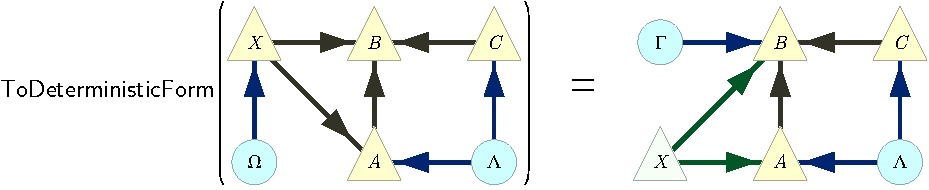
\includegraphics[scale=1]{ExampleToDeterministic.pdf}
%\caption{An example of choosing to illustrate a DAG in deterministic form. The non-root node $B$ lacked a latent parent, so we add one. The latent node $\Omega$ was useless, so we deleted it.}\label{fig:ExampleToDeterministic}
%\end{figure}


A kind of DAG with special importance to use here is a DAG which happens to be in \tred{purely common cause (PCC)} form. A PCC scenario is a two-layer causal structure in which every node is either a ``cause" or an ``effect", such that the only edges in the DAG are those which connect cause nodes to effect nodes. All causal pathways in a PCC DAG have length $1$, i.e. there is precisely one edge in every connected path between any root node and any terminal node in a PCC DAG.

PCC DAGs are important to use because our technique works by first mapping the target causal structure $G$ to a PCC representation, $G'=\NamedFunction{ReduceToPCC}{\!G\!}$ whenever $G$ is not already in PCC form. For pedagogical clarity we choose to delay discussing the details of the $\mathsf{ReduceToPCC}$ until \cref{sec:topcc}. We begin, rather, by illustrating sample derivations of polynomial inequalities on a few \emph{innately} PCC scenarios.

We follow the convention that upper-case letters indicate random variables while lower-case letters indicate some particular value associated with the corresponding random variable. In this convention, for example, a student's score on some exam $X$ might depend probabilistically on the extent of sleep $S$. The Boolean proposition, or {event}, $X\cramp{=}x|S\cramp{=}s$ should be understood as "the students scores $x$ on the exam given a duration of sleep equal to $s$. As conditional propositions form the basis of much of what follows, we \tred{represent conditioning via subscript notation}, such as $x_s$ to indicate the event $X\cramp{=}x | S\cramp{=}s$. 

\purp{NEW CONVENTION: Need to update ALL the figures.} Throughout this article latent random variables are represented by Greek letters $\Lambda\cramp{=}\lambda,\Gamma\cramp{=}\gamma,...,$ whereas observable variables are represented by Roman letters $A\cramp{=}a,B\cramp{=}b,...$ etc. We reserve letters from the \emph{end} of the Roman alphabet to represent variables which are root nodes in the DAG. In graphical depictions we follow the convention of representing latent variables by circles and observable variables by triangles \cite{pusey2014gdag}.

We choose to indicate logical negation by $\NamedFunction{Not}{\!x\!}\equiv\n{x}$ such that $\n{x}$ references the possibility of \emph{any} outcome other than $x$, i.e. $\p{\n{x}}\equiv\p{X\cramp{\neq}x}=1-\p{X\cramp{=}x}$. The negation of a conditional event should be interpreted as any other outcomes given the same settings, such that $\p{\n{x_{s a}}}=\p{X\cramp{\neq}x|S\cramp{=}s,A\cramp{=}a}$.

Note that \tred{logical conjunction is herein represented by default}, such that $\p{x y}$ is the probability of $X\cramp{=}x$ \emph{and} $Y\cramp{=}y$. Logical conjunction is also implicit among all variables appearing in subscript.

Finally, note that \tred{superscript notation indicates a dummy index}, such that $x^2_{s^2 a^1}$ is shorthand for $\parens*{X\cramp{=}x^{(2)}|S\cramp{=}s^{(2)},A\cramp{=}a^{(1)}}$. 



\section{Bell Scenario (New)}

Consider the causal structure associated to the Bell/CHSH \cite{bell1964einstein,Brunner2013Bell,bell1966lhvm,CHSHOriginal} experiment [\citealp{pusey2014gdag}~(Fig.~E\#2), \citealp{WoodSpekkens}~(Fig.~19), \citealp{chaves2014novel}~(Fig.~1), \citealp{BeyondBellII}~(Fig.~1), \citealp{wolfe2015nonconvexity}~(Fig.~2b), \citealp{steeg2011relaxation}~(Fig.~2)], depicted here in \cref{fig:NewBellDAG}. $\brackets{A,B,X,Y}$ are all observable variables, and $\Lambda$ is the latent common cause of $A$ and $B$.

\begin{figure}[H]
\centering
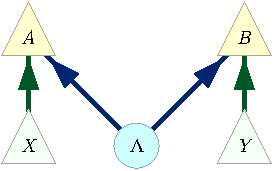
\includegraphics[scale=1]{NewBellDAG.pdf}
\caption{The causal structure of the Bell scenario. The local outcomes of Alice's and Bob's experimental probing is assumed to be a function of some latent common cause, in addition to their independent local experimental settings.}\label{fig:NewBellDAG}
\end{figure}


%Without loss of generality let's assume that the values $\Lambda\mathopen{=}\lambda$ are drawn from some (possibly infinite, possibly continuous) set $\lambda\in\Omega$. 
The assumption of this causal structure dictates that
\begin{align}\begin{split}\label{eq:bellstructureNEW}
%\p{x y s t | \lambda a b}=\p{x_{\lambda a} y_{\lambda b} s_x t_y}
\p{a_{\lambda x y}}=\p{a_{\lambda x}} \,,\; \p{b_{\lambda x y}}=\p{b_{\lambda y}} \,,\; \p{\lambda x y}=\p{\lambda}\p{x}\p{y} \,,%\quad\text{and hence}\quad \p{x y s t | \lambda a b}=\p{x_{\lambda a} y_{\lambda b} s_x t_y}\,,
%=\p{x_{s|\lambda}}\p{y_{t|\lambda}}
\end{split}\end{align}
and hence
\begin{align}\begin{split}\label{eq:bellintegrationNEW}
&\p{a b | \lambda x y}=\p{a_{\lambda x} b_{\lambda y}}\,,\quad\text{and accordingly}\quad \p{a b | x y}=\sum\limits_{{\lambda\in \norm{\Lambda}}}\p{a_{\lambda x} b_{\lambda y}}\p{\lambda}.
\end{split}\end{align}


\begin{prop}\label{prop:rawCHnew}
The Bell causal structure (\cref{fig:NewBellDAG}) implies that
\begin{align*}
\p{a^1 b^1|x^1 y^1} \p{a^2 b^2|x^2 y^2}
\leq
{
\p{\n{a^3} \n{b^3}|x^1 y^1}
+\p{a^1|x^1} \p{a^2 b^3|x^2 y^1}
+\p{b^1|y^1} \p{a^3 b^2|x^1 y^2}
}
\end{align*}
\end{prop}
\begin{proof}
We use the causal structure to consider various counterfactual propositions, which we collect into a logical tautology as follows.
\begin{align}\label{eq:bell2structaut}
\NamedFunction{And}{ a^1_{x^1 \lambda ^1} , b^1_{y^1 \lambda ^1} , a^2_{x^2 \lambda ^2} , b^2_{y^2 \lambda ^2} }
\implies 
\NamedFunction{Or}{
    \NamedFunction{And}{ \n{a^3_{x^1 \lambda ^2}} , \n{b^3_{y^1 \lambda ^2}} } ,\\
    \NamedFunction{And}{ b^1_{y^1 \lambda ^1} , a^3_{x^1 \lambda ^2} , b^2_{y^2 \lambda ^2} } ,\\
    \NamedFunction{And}{ a^1_{x^1 \lambda ^1} , a^2_{x^2 \lambda ^2} , b^3_{y^1 \lambda ^2} }
}
\end{align}
Next, we convert the tautology to an inequality via two rules:
\begin{compactenum}
\item As the antecedent always implies the consequent, the probability of the antecedent is necessarily less-than-or-equal-to the probability of the consequent. If $j \cramp{\scriptstyle \implies} k$ then $\p{j}\leq\p{k}$.
\item The probability of a disjunction of events is less-than-or-equal-to the sum of the probabilities of the individual events, i.e. ${\p{j\lor k}=\p{j}+\p{k}-\p{j,k}\leq \p{j}+\p{k}}$.
\end{compactenum}
The inequality which corresponds to \cref{eq:bell2structaut} is
\begin{align}\label{eq:bell2structineq}
\p{a^1_{x^1 \lambda ^1} , b^1_{y^1 \lambda ^1}} \p{a^2_{x^2 \lambda ^2} , b^2_{y^2 \lambda ^2}}
\leq
{
\p{\n{a^3_{x^1 \lambda ^2}} , \n{b^3_{y^1 \lambda ^2}}}
+\p{b^1_{y^1 \lambda ^1}} \p{a^3_{x^1 \lambda ^2} , b^2_{y^2 \lambda ^2}}
+\p{a^1_{x^1 \lambda ^1}} \p{a^2_{x^2 \lambda ^2} , b^3_{y^1 \lambda ^2}}
}
\end{align}
Note that we have factored terms in \cref{eq:bell2structineq} according to distinct counterfactual instances of \emph{causes}. This is the key step in deriving polynomial inequalities. The distinct counterfactual instances are perhaps best seen by rewriting \cref{eq:bell2structineq} in a manner which does not assume a particular causal structure, namely
\begin{align}\label{eq:bell2operineq}
\p{a^1 b^1|x^1 y^1 \lambda ^1} \p{a^2 b^2|x^2 y^2 \lambda ^2}
\leq
{
\p{\n{a^3} \n{b^3}|x^1 y^1 \lambda ^2}
+\p{a^1|x^1 \lambda ^1} \p{a^2 b^3|x^2 y^1 \lambda ^2}
+\p{b^1|y^1 \lambda ^1} \p{a^3 b^2|x^1 y^2 \lambda ^2}
}
\end{align}
which we can marginalize both sides over all  $\lambda^1$ and $\lambda^2$ to obtain \cref{prop:rawCHnew}.
\end{proof}

As both \cref{eq:bell2structaut,eq:bell2operineq} can be inferred from \cref{eq:bell2structineq}, we shall include only inequalities written in terms of single-effect counterfactuals in subsequent proofs of polynomial inequalities.



Note that as a general matter, polynomial inequalities can be relaxed into interesting special cases by \emph{disregarding} some outcome possibilities, either by imagining the outcome to be \emph{impossible} or \emph{inevitable}. For example, the special case $a^3\to \mathsf{False}$ means we imagine  $a^3\not\in \norm{A}$, the ramifications being $\p{\n{a^3} \n{b^3}|x^1 y^1}\to\p{\n{b^3}|x^1 y^1}$ and $\p{a^3 b^2|x^1 y^2}\to 0$ etc. Similarly, the special case $\brackets{a^1,b^1}\to \mathsf{True}$ reduces \cref{prop:rawCHnew} into
\begin{align}\label{eq:preCHnew}
\p{a^2 b^2|x^2 y^2}
\leq
{
\p{\n{a^3} \n{b^3}|x^1 y^1}
+\p{a^2 b^3|x^2 y^1}
+\p{a^3 b^2|x^1 y^2}
}\,.
\end{align}
A further special case of \cref{eq:preCHnew} is achieved by selecting $a^2\to a$, $a^3\to \n{a}$, $b^2\to b$, $b^3\to \n{b}$, yielding
\begin{align}\label{eq:preCHnew2}
\p{a b|x^2 y^2}
\leq
{
\p{a b|x^1 y^1}
+\p{a \n{b}|x^2 y^1}
+\p{\n{a} b|x^1 y^2}
}\,.
\end{align}
We may eliminate negation notation entirely from \cref{eq:preCHnew2} by noting that $\p{a \n{b} | x y} = \p{a | x y}-\p{a b | x y} = \p{a | x}-\p{a b | x y}$ etc, where the last equality makes use of the causal structure per \cref{eq:bellstructureNEW}. Hence
\begin{prop}\label{prop:CHnew}
The Bell causal structure (\cref{fig:NewBellDAG}) implies that
\begin{align*}
\p{a b|x^2 y^2}+\p{a b|x^2 y^1}+\p{a b|x^1 y^2}
\leq
{
\p{a b|x^1 y^1}
+\p{a |x^2}
+\p{b |y^2}
}
\end{align*}
\end{prop}
which is simply the Clauser-Horne (CH) inequality \cite{CHInequality} for the Bell scenario. The CH inequality is the \emph{unique} Bell inequality (up to permutations) for the Bell scenario if $\brackets{A,B,X,Y}$ are all binary, and hence the CH inequality is a necessary and sufficient criterion to ascertain if correlations are compatible with that Bell scenario variant.





\section{Triangle and S15 Scenarios \purp{Need real name?} (New)}

Consider the causal structure depicted here in \cref{fig:NewS15DAG}, which corresponds to ``interesting" DAG \#15 in Ref. \cite{pusey2014gdag}. $\brackets{A,B,C,X}$ are all observable variables, $\brackets{A,B,C}$ are all pairwise-correlated by a common cause although only the common cause of $A$ and $B$ is observable.


\begin{figure}[H]
\centering
\begin{minipage}[b]{0.49\linewidth}
\centering
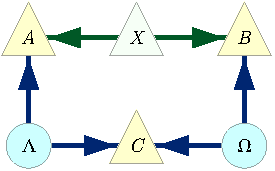
\includegraphics[scale=1]{NewS15DAG.pdf}
\caption{The causal structure of the S15 scenario.}\label{fig:NewS15DAG}
\end{minipage}
\hfill
\begin{minipage}[b]{0.49\linewidth}
\centering
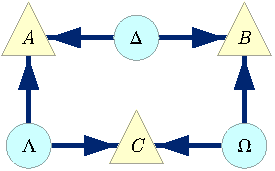
\includegraphics[scale=1]{NewTriDAG.pdf}
\caption{The causal structure of the Triangle scenario.}\label{fig:NewTriDAG}
\end{minipage}
\end{figure}

The assumption of causal structure per \cref{fig:NewS15DAG} dictates that
\begin{align}\begin{split}\label{eq:s15structure}
%\p{x y z | a b c}=\p{x_{c a}  y_{a b}  z_{b c}}
\p{a_{x \lambda \omega}}=\p{a_{x \lambda}} \,,\; \p{b_{x \lambda \omega}}=\p{b_{x \omega}} \,,\; \p{c_{x \lambda \omega}}=\p{c_{\lambda \omega}} \,,\quad\text{and hence}\quad \p{a b c | x \lambda \omega}=\p{a_{x \lambda} b_{x \omega} c_{\lambda \omega}}\,,
\end{split}\end{align}
and accordingly, 
\begin{align}\label{eq:s15integration}
&\p{a b c | x}=\sum\limits_{\omega\in \norm{\Omega}} \sum\limits_{\lambda\in \norm{\Lambda}} \p{a_{x \lambda} b_{x \omega} c_{\lambda \omega}}\p{\lambda}\p{\omega}.
\end{align}
The Triangle scenario in \cref{fig:NewTriDAG} is clearly just the S15 scenario under ignorance about the distribution of $X$; i.e. $X\to \Delta$, an observable variable becomes hidden. This mapping is useful to us, as we we can derive polynomial causal compatibility criteria for both scenarios simultaneously. Indeed, \cref{eq:s15structure,eq:s15integration} apply just as well to the Triangle scenario under the substitution $x\to \delta$. 
The assumption of causal structure per \cref{fig:NewTriDAG} dictates that $\p{a b c | \delta \lambda \omega}=\p{a_{\delta \lambda} b_{\delta \omega} c_{\lambda \omega}}$, and accordingly that
\begin{align}\label{eq:triintegration2}
&\p{a b c}=\sum\limits_{\delta\in \norm{\Delta}}\p{a b c | \delta}= \sum\limits_{\delta\in \norm{\Delta}}\sum\limits_{\omega\in \norm{\Omega}} \sum\limits_{\lambda\in \norm{\Lambda}} \p{a_{x \lambda} b_{x \omega} c_{\lambda \omega}}\p{\lambda}\p{\omega}\p{\delta}.
\end{align}

\begin{prop}\label{prop:s15d2}
The S15 causal structure (\cref{fig:NewS15DAG}) implies that
\begin{align*}
\p{a^1 b^1 c^1|x^1} \p{a^2 b^2 c^2|x^2}
\leq
{
\p{c^1} \p{\n{a^3} \n{b^3} c^2|x^1}
+\p{a^2|x^2} \p{a^1 b^3|x^1}
+\p{b^2|x^2} \p{a^3 b^1|x^1}
}
\end{align*}
\end{prop}
\begin{proof}
\begin{align}\label{eq:s15d2structineq}
\p{a^1_{x^1 \lambda^1} b^1_{x^1 \omega^1} c^1_{\omega^1 \lambda^1}} \p{a^2_{x^2 \lambda^2} b^2_{x^2 \omega^2} c^2_{\omega^2 \lambda^2}}
\leq
\lparens{
\hphantom{+}\p{\n{a^3_{x^1 \lambda^2}} \n{b^3_{x^1 \omega^2}} c^2_{\omega^2 \lambda^2}} \p{c^1_{\omega^1 \lambda^1}}
\\+\p{a^3_{x^1 \lambda^2} b^1_{x^1 \omega^1}} \p{b^2_{x^2 \omega^2}}
\\+\p{a^1_{x^1 \lambda^1} b^3_{x^1 \omega^2}} \p{a^2_{x^2 \lambda^2}}
}\qedhere
\end{align}
\end{proof}
In turn, and for free, we also have
\begin{prop}\label{prop:trid2}
The Triangle causal structure (\cref{fig:NewTriDAG}) implies that
\begin{align*}
\p{a^1 b^1 c^1} \p{a^2 b^2 c^2}
\leq
{
\p{c^1} \p{\n{a^3} \n{b^3} c^2}
+\p{a^2} \p{a^1 b^3}
+\p{b^2} \p{a^3 b^1}
}
\end{align*}
\end{prop}
which follows from \cref{prop:s15d2} by marginalization over $x$, which is not observable in the Triangle scenario.

\clearpage
Similarly, we have
\begin{prop}\label{prop:s15d3}
The S15 causal structure (\cref{fig:NewS15DAG}) implies that
\begin{align*}
\p{a^1 b^1 c^1|x^1} \p{a^2 b^2 c^2|x^2} \p{a^3 b^3 c^3|x^3}
\leq
\lparens{
\hphantom{+}\p{\n{a^4} \n{b^4} \n{c^4}|x^1} \p{\n{a^5} \n{b^5} \n{c^5}|x^2}
\\+\p{b^3|x^3} \p{b^2 c^4|x^2} \p{a^1 b^1 c^1|x^1}
\\+\p{c^2} \p{b^5 c^3|x^2} \p{a^1 b^1 c^1|x^1}
\\+\p{a^3|x^3} \p{a^1 c^5|x^1} \p{a^2 b^2 c^2|x^2}
\\+\p{c^1} \p{a^4 c^3|x^1} \p{a^2 b^2 c^2|x^2}
\\+\p{a^2|x^2} \p{a^1 b^4|x^1} \p{a^3 b^3 c^3|x^3}
\\+\p{b^1|x^1} \p{a^5 b^2|x^2} \p{a^3 b^3 c^3|x^3}
}
\end{align*}
\end{prop}
\begin{proof}
\begin{align}\label{eq:s15d3structineq}
\p{a^1_{x^1 \lambda^1} b^1_{x^1 \omega^1} c^1_{\omega^1 \lambda^1}} \p{a^2_{x^2 \lambda^2} b^2_{x^2 \omega^2} c^2_{\omega^2 \lambda^2}} \p{a^3_{x^3 \lambda^3} b^3_{x^3 \omega^3} c^3_{\omega^3 \lambda^3}}
\leq
\lparens{
\hphantom{+}\p{\n{a^4_{x^1 \lambda^3}} \n{b^4_{x^1 \omega^2}} \n{c^4_{\omega^2 \lambda^3}}} \p{\n{a^5_{x^2 \lambda^1}} \n{b^5_{x^2 \omega^3}} \n{c^5_{\omega^3 \lambda^1}}}
\\+\p{a^1_{x^1 \lambda^1} b^4_{x^1 \omega^2}} \p{a^3_{x^3 \lambda^3} b^3_{x^3 \omega^3} c^3_{\omega^3 \lambda^3}} \p{a^2_{x^2 \lambda^2}}
\\+\p{a^1_{x^1 \lambda^1} c^5_{\omega^3 \lambda^1}} \p{a^2_{x^2 \lambda^2} b^2_{x^2 \omega^2} c^2_{\omega^2 \lambda^2}} \p{a^3_{x^3 \lambda^3}}
\\+\p{a^5_{x^2 \lambda^1} b^2_{x^2 \omega^2}} \p{a^3_{x^3 \lambda^3} b^3_{x^3 \omega^3} c^3_{\omega^3 \lambda^3}} \p{b^1_{x^1 \omega^1}}
\\+\p{b^2_{x^2 \omega^2} c^4_{\omega^2 \lambda^3}} \p{a^1_{x^1 \lambda^1} b^1_{x^1 \omega^1} c^1_{\omega^1 \lambda^1}} \p{b^3_{x^3 \omega^3}}
\\+\p{a^4_{x^1 \lambda^3} c^3_{\omega^3 \lambda^3}} \p{a^2_{x^2 \lambda^2} b^2_{x^2 \omega^2} c^2_{\omega^2 \lambda^2}} \p{c^1_{\omega^1 \lambda^1}}
\\+\p{b^5_{x^2 \omega^3} c^3_{\omega^3 \lambda^3}} \p{a^1_{x^1 \lambda^1} b^1_{x^1 \omega^1} c^1_{\omega^1 \lambda^1}} \p{c^2_{\omega^2 \lambda^2}}
}\qedhere
\end{align}
\end{proof}
Again, in turn,and for free, we also have
\begin{prop}\label{prop:trid3}
The Triangle causal structure (\cref{fig:NewTriDAG}) implies that
\begin{align*}
\p{a^1 b^1 c^1} \p{a^2 b^2 c^2} \p{a^3 b^3 c^3}
\leq
\lparens{
\hphantom{+}\p{\n{a^4} \n{b^4} \n{c^4}} \p{\n{a^5} \n{b^5} \n{c^5}}
\\+\p{b^3} \p{b^2 c^4} \p{a^1 b^1 c^1}
\\+\p{c^2} \p{b^5 c^3} \p{a^1 b^1 c^1}
\\+\p{a^3} \p{a^1 c^5} \p{a^2 b^2 c^2}
\\+\p{c^1} \p{a^4 c^3} \p{a^2 b^2 c^2}
\\+\p{a^2} \p{a^1 b^4} \p{a^3 b^3 c^3}
\\+\p{b^1} \p{a^5 b^2} \p{a^3 b^3 c^3}
}
\end{align*}
\end{prop}
which again follows by marginalization over $x$, this time via from \cref{prop:s15d3}.



A special case of \cref{prop:trid3} is
\begin{prop} \label{prop:FritzF2new}
The Triangle causal structure (\cref{fig:NewTriDAG}) implies that
\begin{align*}\begin{split}
\p{a}\p{b}\p{c}\leq&+\p{\n{a},\n{b},\n{c}}+ \p{a}\p{b,c} + \p{b}\p{c,a}+ \p{c}\p{a,b}.
\end{split}\end{align*}
\end{prop}
\begin{proof}
First, let $\brackets{a^5,b^5,c^5}\to\mathsf{False}$ and $\brackets{a^2,a^3,b^1,b^3,c^1,c^2}\to\mathsf{True}$. This yields
\begin{align}
\p{a^1 } \p{b^2} \p{c^3}
\leq
{
\hphantom{+}\p{\n{a^4} \n{b^4} \n{c^4}} 
+\p{b^2 c^4} \p{a^1}
+\p{a^4 c^3} \p{b^2}
+\p{a^1 b^4} \p{c^3}
}
\end{align}
which reduces to \cref{prop:FritzF2new} by further substituting $a^4\to a^1\to a$, $b^4\to b^2\to b$, and $c^4\to c^3\to c$.
\end{proof}


A consequence of \cref{prop:FritzF2new} is that the W-type distribution
\begin{align}\label{eq:wdistributionnew}
p_{\text{W}}\parens{a,b,c}=\begin{cases}\tfrac{1}{3}&\text{if }\; a+b+c=1 \\ 0&\text{otherwise}\end{cases}
\end{align}
is found to be incompatible with the Triangle scenario, where $a,b,c\in\brackets{0,1}$. The W-distribution states that the in any event in which $A,B,C$ are observed, precisely one of them will be found to equal $1$ while the other two will equal $0$. The identity of the variable which takes the value $1$ is uniformly random. In informal but intuitive notation, the W-type distribution is ${\nicefrac{1}{3}[100]+\nicefrac{1}{3}[010]+\nicefrac{1}{3}[001]}$.
To see how this distribution is incompatible with \cref{prop:FritzF2new}, note that for three \emph{identically distributed} (but not independent) binary variables a further special case of \cref{prop:FritzF2new} is
\begin{align*}\begin{split}
&\hspace{-6ex}\p{A\cramp{=}1}^3\leq \p{A\cramp{=}B\cramp{=}C\cramp{=}0} + 3\times\p{A\cramp{=}1,B\cramp{=}1}\p{C\cramp{=}1}.
\end{split}\end{align*}
For the W-distribution ${\p{A\cramp{=}B\cramp{=}C\cramp{=}0}=0}$, and also ${\p{A\cramp{=}1,B\cramp{=}1}=0}$, yet ${\p{A\cramp{=}1}=\nicefrac{1}{3}}$. As ${(\nicefrac{1}{3})^3\nleq 0}$ we have proven that the W-type distribution is incompatible with the Triangle scenario.



\section{Failure of Entropic Inequalities \purp{switch notation}}

It is interesting to note that entropic inequalities \cite{fritz2013marginal,chaves2014novel,chaves2014informationinference} fail to recognize the W-type distribution as incompatible with the Triangle scenario, the polynomial inequalities derivable through our method are capable of doing so. To reiterate from the abstract, enumeration of entropic inequalities is considered state-of-the-art derivation of necessary albeit insufficient causal structure compatibility criteria \cite{pusey2014gdag}. The insufficiency is a pressing concern in quantum information theory as there are uniquely-quantum distributions which cannot be certified as non-classical by means of entropic inequalities, for instance in the Triangle scenario \citep[Prob. 2.17]{fritz2012bell}. Many interesting quantum correlation are identified by entropic inequalities, however \cite{SchumacherInequality,chaves2012entropic}. 

%The entropic inequalities associated with the Bell scenario\footnote{Generally a non-trivial entropic inequality is defined as one that takes into account the causal structure somehow. There are no such entropic inequalities for Bell scenarios, so the inequality listed here is Shannon-type, and can be derived from nothing more than the assumption of joint measurability.} are given by
%\begin{align}\begin{split}\label{eq:entropicCHSH}
%&H\parens{A_1,B_1}+H\parens{A_0}+H\parens{B_0}
%\\&\leq H\parens{A_0,B_0}+H\parens{A_0,B_1}+H\parens{A_1,B_0}
%\end{split}\end{align}
%and its permutations \cite{chaves2014novel,chaves2012entropic}.

The entropic inequalities associated with the Triangle scenario are given by 
\begin{align}\label[eqs]{eq:entropicineqs}\begin{split}
&I\parens{A:B}+I\parens{A:C}\leq H\parens{A}
\\\text{and }\quad&I\parens{A:B}+I\parens{A:C}+I\parens{B:C}\leq H\parens{A,B}-I\parens{A:B:C}
\\\text{and }\quad & I\parens{A:B}+I\parens{A:C}+I\parens{B:C}\leq\frac{H\parens{A}+H\parens{B}+H\parens{C}}{2}-I\parens{A:B:C}
\end{split}\end{align}
and their permutations \cite{chaves2014novel,Chaves2015infoquantum,pusey2014gdag,steudel2010ancestors}.

Note that bipartite mutual information may be understood as $I\parens{A:B}\equiv H\parens{A}+H\parens{B}-H\parens{A,B}$ and tripartite mutual information is defined as $I\parens{A,B,C}\equiv H\parens{A}+H\parens{B}+H\parens{C}-H\parens{A,B}-H\parens{A,C}-H\parens{B,C}+H\parens{A,B,C}$. It is straightforward to demonstrate that the W-type distribution given in \cref{eq:wdistributionnew} satisfy \cref{eq:entropicineqs}.





\section{Deriving inequalities algorithmically}

As evidenced, we derive polynomial inequalities in the observable variables by constructing logical tautologies (and their associated inequalities) in terms of conditional propositions. From the previous examples examples it should be clear why the tautologies make use of PCC format. Therefore, the preliminary step for deriving polynomial inequalities from $G$ is $\mathsf{ReduceToPCC}$ if the scenario isn't already innately PCC.

In algorithmically deriving polynomial inequalities we elect to sacrifice some generality in exchange for simplicity. In particular, we herein limit our consideration to tautologies of the ``supplemented excluded middle" (SEM) form. An excluded-middle (EM) tautology follows the following format: 
%\begin{align}
%Q1 \lor Q2 \lor Q3 \lor...\lor \parens*{\n{Q1}\land\n{Q2}\land\n{Q3}\land...}
%\end{align}
\begin{align}
\NamedFunction{Or}{Q1 , Q2 , Q3 ,..., \NamedFunction{And}{\n{Q1} ,\n{Q2},\n{Q3},...}}
\end{align}
An SEM tautology intersperses an EM tautology with a bunch of ``known" proposition, such as the following:
\begin{align}
%P1\land P2 \land P3 \land ... \implies \parens*{Q1\land P2\land P3} \lor \parens*{Q2\land P1\land P3} \lor \parens*{Q3\land P1\land P2} \lor...\lor \parens*{\n{Q1}\land\n{Q2}\land\n{Q3}\land ...}
\NamedFunction{And}{P1, P2 , P3 , ...} \implies 
\NamedFunction{Or}{
  \NamedFunction{And}{Q1, P2 , P3 , ...}
\\\NamedFunction{And}{P1, Q2 , P3 , ...}
\\\NamedFunction{And}{P1, P2 , Q3 , ...}
\\\NamedFunction{And}{\n{Q1} ,\n{Q2},\n{Q3},...}
}
\end{align}
The inequalities in terms of conditional events (such as \cref{eq:bell2structineq,eq:s15d2structineq,eq:s15d3structineq}) must satisfy the following requirements in order to correspond to SEM tautologies and still admit marginalization over the latent variables:
\begin{compactitem}[$\bullet$]
\item Every event on the right hand side of the inequality but not on the left hand side should appear negated in the final term on the left hand side. Such events are the ``unknowns" in the supplemented tautology of the excluded middle. 
%We've been highlighting them in the latent-complete inequalities presented here. 
We call the final term on the right hand side the ``closure" term, as it is closes the excluded middle tautology.

\item Every ``unknown" event (i.e. every event on the right hand side of the inequality but not on the left hand side) should appear in precisely \emph{one} non-closure term on the left hand side. No two such events are allowed in any single term, aside from the closure term, as this would (typically) break the tautology.\footnote{Any tautology of the form $\NamedFunction{And}{\_...}\cramp{\scriptstyle\implies}\NamedFunction{Or}{\NamedFunction{And}{\_...},\NamedFunction{And}{\_...},...}$ corresponds to a legitimate inequality. The SEM tautology is only the easiest to construct, but others are also possible.}

\item In every term, on both sides of the inequality, all instances of a latent variable with common dummy index must be restricted to the same joint probability. This is necessary in order to marginalize over the latent variables pursuant to the causal structure.
\end{compactitem}

While not strictly necessary, in order to make the inequality as compelling as possible one should ensure that every event on the left hand side should also be referenced on the right hand side. If one finds an inequality lacking this property, one can tighten it by using the special in which all such events are set to $\mathsf{True}$. Such choice substitution increases the probability of the left hand side without affecting the right hand side.

Note that these polynomial inequalities are not related whatsoever to the polynomial Bell inequalities recently introduced by \citet{ChavesPolynomial} and \citet{RossetNetworks}, nor to the interventional inequalities of \citet{kang2007polynomialconstraints} and \citet{steeg2011relaxation}.



\section{Reduction to Purely Common Cause (New)}\label{sec:topcc}


Reducing a DAG $G$ to purely common cause form consists of two transformations in succession.
\begin{compactenum}
\item Every causal pathway is replaced with a direct causal connection. This transformation adds edges to $G$ until every root node is directly connection to every one of its causal descendants.\\ ${A\text{-directed-path-to-}B \text{ becomes } A \to B \text{ whenever } A\in \NamedFunction{RootVars}{\!G\!}}$.
\item Edges which do not initiate from root nodes are purged. This transformation deletes edges from $G$ until the only remaining edges are those connected nodes from the ``causes" layer to nodes in the ``effects" layer. \\ ${U \to V \text{ becomes } U \not\to V \text{ whenever } U\not\in \NamedFunction{RootVars}{\!G\!}}$.
\end{compactenum}

\begin{figure}[H]
\centering
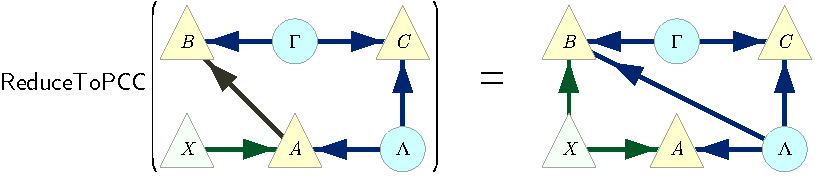
\includegraphics[scale=1]{ExampleToPCCnodel.pdf}
\caption{An example of forcing a DAG into purely common cause (PCC) form. The DAG is relaxed under this transformation. Note the addition of edges initiating from $X$ and $\Lambda$, and the delete of an edge between the two non-root nodes $A\to B$.}\label{fig:ExampleToPCC}
\end{figure}

We will shortly prove that reducing to PCC is generally a relaxation of $G$; any causal compatibility criteria applicable to $G'=\NamedFunction{ReduceToPCC}{\!G\!}$ is therefore also applicable to $G$. 

Many observationally equivalent causal structures can have the same PCC reduction, for example $G\neq 
H$ but $\NamedFunction{ReduceToPCC}{\!G\!}= \NamedFunction{ReduceToPCC}{\!H\!}$. If two structures have the same PCC reduction we call them \tred{equivalent under PCC reduction}. If a structure is observationally equivalent to its PCC reduction then we deem that structure \emph{observationally invariant under PCC reduction}, or \tred{PCC-lossless} for short. Determining if a DAG is PCC-lossless is addressed in \cref{prop:PCClossless}.

Mapping genuine causal structures into their PCC reductions has previously been recognized as an effective technique in causal inference, see Refs. \citep[Thm. 2.4]{fritz2012bell} and \citep[Sec. 5]{BilocalCorrelations}. Our inequalities apply to the PCC reductions, and hence only indirectly to their generating causal structures. Causal structures which are isomorphic to their PCC reductions, including the Triangle scenario, have been studied at length by \citet{fritz2012bell}; the connection to more general causal structures is further elucidated in Ref. \cite{BeyondBellII}.

Innately PCC causal structures where the root nodes are all latent variables are known as ``correlation scenarios" \cite{fritz2012bell}. Quantum physicists may wish to note the following result \citep[Thm.~3.8]{fritz2012bell}: Correlation scenarios which are star graphs \citep[Fig.~6]{fritz2012bell} do not admit uniquely-quantum (non-classical) probability distributions. That is, replacing classical latent variables with quantum states does not expand the set of possibly-observable distributions for such correlation structures. Consequently, all general causal structures which are star graphs under PCC reduction also do not admit quantum probability distributions \purp{no longer 100\% obvious}. The classification of causal structures which admit non-classical probability distributions has been addressed in further detail by \citet{pusey2014gdag}. 

\section{Recognizing observationally equivalent DAGs}

\purp{Notes to self: Discuss add-edge theorem, then subtract edge theorem, then why the second step of ReduceToPCC is observationally invariant, then give the criterion for PCC-lossless, then comment about matching-up latent variables between causal structures.}

%Without loss of generality we herein consider only deterministic DAGs where all latent variables are parentless. \purp{Either prove this, or remove it. If not invoked we should discuss adding edges TO latent variables.}

We intuitively expect that an edge $A\to B$ can be added to DAG $G$ while leaving $G$ observationally invariant if the new connection does introduce any new information about observable variables to $B$. If the added connection does inform $B$ about some observable $C$, that's still ok so long as if the new informational cannot be exploited to increase the correlation between $B$ and $C$. We formalize this notion now.

\begin{theorem}\label{theo:edgeadding}
Let $\bm{O}$ be the set of observables nodes in a DAG $G$.
Let $\bm{X}=\lparens{X s.t. \NamedFunction{pa}{\!B\!}\in\NamedFunction{SS}{\!A|X\!}}$ be the set of nodes in $G$ relative to which $\NamedFunction{pa}{\!B\!}$ comprise a \emph{sufficient statistic} for node $A$.
Let $\bm{Y}=\NamedFunction{UC_{B}}{\!G\!}$ be the set of nodes in $G$ which have potentially \emph{unlimited correlation} with $B$.
Then, an edge $A\to B$ can be added to DAG $G$ while leaving $G$ observationally invariant if and only if (prior to adding the edge) $\bm{O}\subseteq \bm{X}\cup \bm{Y}$.
\end{theorem}

Let's define the concepts in \cref{theo:edgeadding}, and make them operationally useful. $Z$ is (or ``are") a sufficient statistic for $A$ relative to $X$ , hereafter $Z\in\NamedFunction{SS}{\!A|X\!}$ if all inferences about $X$ knowing $A$ are also possible without knowing $A$ but with knowing $Z$ instead. In other words, learning $A$ can never teach anything new about $X$ if $Z$ is already known. %This is guaranteed if $X$ and $A$ are conditionally independent given $Z$, so if $X$ and $A$ are $d$-separated by $Z$, then $Z\in\NamedFunction{SS}{\!A|X\!}}$ 

$Z\in\NamedFunction{SS}{\!A|X\!}$ if $A$ or $X$ are completely predictable given $Z$, or if $Z$ contains a Markov Blanket (MB) for $\bm{V}$ such that $A\in \bm{V}$ while $X\not\in \bm{V}$, 
which screens off $X$ from $A$. These need further definition.

In a deterministic DAG, $V$ is perfectly predictable given its parents, that is, $\NamedFunction{pa}{\!V\!}\in\NamedFunction{SS}{\!V|\text{anything}\!}$. Moreover, the parents of a latent variable are perfectly predictable ``given" the latent variable, that is, ${\Lambda\in\NamedFunction{SS}{\!\NamedFunction{pa}{\!\Lambda\!}|\text{anything}\!}}$. 

By composing these two rules we can identify the complete set of nodes which are perfectly predicable from $Z$ alone. \purp{do so!}

It is convenient to assume that all latent variables are parentless in the DAG. (This can actually be done without loss of generality; a DAG with non-root latent nodes can be transformed into an observationally equivalent one by rerouting all parents of the latent node directly to all its children. \purp{proof...}) In a latent-parentless deterministic DAG the node $V$ is completely predictable from $Z$ alone if and only if $V$ is an \emph{exclusive descendant} of $Z$. $V$ is an exclusive descendant of $Z$ if the intersection of [the ancestors of $V$] with [the non-ancestors of $Z$] is a subset of {[the descendants of $Z$]}. 
 
The Markov Blanket for $V$, $\NamedFunction{MB}{\!V\!}$ is the set of all of $V$'s children, parents, and co-parents. The Markov Blanket is so defined because $V$ is conditionally independent \emph{everything} given $\NamedFunction{MB}{\!V\!}$. For our purposes, ${\NamedFunction{MB}{\!V\!}\in\NamedFunction{SS}{\!V|\text{anything-but-}V\!}}$.

Nodes $A$ and $B$ have potentially unlimited correlation in a DAG if and only if $A \leadsto  B$ (and $A$ has at least one latent parent), or $A\leadsto B$ (and $B$ has at least one latent parent), or the exists a latent $\Lambda$ such that $\Lambda\leadsto A$ and $\Lambda\leadsto B$.
The notation $A \leadsto  B$ denotes the existence of a directed path from node $A$ to node $B$, where any intermediate nodes are latent \cite{pusey2014gdag}.

Using these definitions, we can now consider special cases of \cref{theo:edgeadding}.
\begin{corollary}\label{cor:edgeaddingSS}
An edge $A\to B$ can be added to some DAG $G$ while leaving $G$ observationally invariant if $\NamedFunction{pa}{\!B\!}$ are a sufficient statistic for $A$ relative to all observable nodes.
As such, the edge $A\to B$ can always be added whenever $A$ is perfectly predictable given $\NamedFunction{pa}{\!B\!}$.
Furthermore, the edge $\Lambda\to B$ can be also always be added when $\Lambda$ is latent if $\NamedFunction{pa}{\!B\!}$ contains a Markov Blanket (MB) for some node-set $\bm{V}$ such that $\Lambda\in \bm{V}$ while no observable variables are inside $\bm{V}$. 
\end{corollary}

We can also define an analogous condition for when an edge can be removed from a DAG without impacting it observationally.
\begin{theorem}\label{theo:edgedropping}
An edge $A\to B$ can be dropped from DAG $G$ to form $G'$ such that $G$ and $G'$ are observationally equivalent if and only if the edge $A\to B$ can be added (back) to $G'$ while leaving $G'$ observationally invariant per \cref{theo:edgeadding}.
\end{theorem}

Recall now the two steps of the transformation $\mathsf{ReduceToPCC}$. Imagine after the first step is finished, that an edge $A\to B$ remains, where $A$ is not a root node. Have directly connected all causal pathways, we know that $\NamedFunction{pa}{\!A\!}\subseteq\NamedFunction{pa}{\!B\!}$. As such, $\NamedFunction{pa}{\!B\!}\in\NamedFunction{SS}{\!A|\text{anything}\!}$, that is to say, $A$ is perfectly predictable given the parents of $B$. By \cref{cor:edgeaddingSS}, therefore, if the edge $A \to B$ were not in the DAG, we would be able to observationally invariantly add it. By \cref{theo:edgedropping}, therefore, removing the edge does not observational impact the DAG. Indeed, the second step of $\mathsf{ReduceToPCC}$ leaves the post-first-step DAG observationally invariant. This allows us to quickly determine if a DAG is PCC-lossless.

\begin{prop}\label{prop:PCClossless}
A DAG $G$ is PCC-lossless if every new edge in $\NamedFunction{ReduceToPCC}{\!G\!}$ relative to $G$ can be accounted for by adding edges to $G$ while leaving $G$ observationally invariant, pursuant to \cref{theo:edgeadding}.
\end{prop}



\begin{comment}
---------------
\section{old toPCC stuff, to be deleted}

In order to understand how reduction to purely common cause (PCC) form impacts a causal structure observationally, it is helpful to identify certain fundamental transformations one can perform on a DAG, many of which leave the DAG observationally invariant. 

\begin{itemize}[$\bullet$]

\item Bypass all latent variables, $\mathsf{BypassLatents}$. For every latent variable which has parent nodes in $G$,  $\NamedFunction{BypassLatents}{\!G\!}$ adds edges to $G$ connecting the parents of the latent variable to the children of the variable. This transformation leaves the DAG observationally invariant, see Thm. 26.3 and its proof in Ref. \cite{pusey2014gdag}. See \cref{fig:ExampleBypassLatents} for an example.
\begin{figure}[h]
\centering
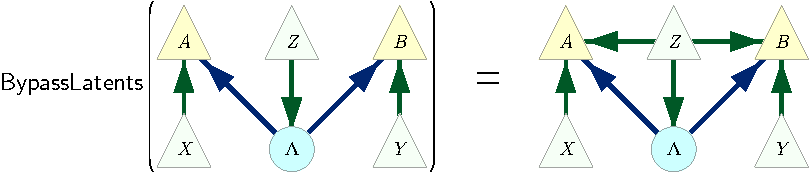
\includegraphics[scale=1]{ExampleBypassLatents.pdf}
\caption{An example of bypassing latent variables. The latent variable $\Lambda$ had a parent $Z$, so we connected $Z$ directly to $\Lambda$'s children.}\label{fig:ExampleBypassLatents}
\end{figure}

\item Make all latent variables parentless, $\mathsf{OrphanLatents}$. This operation \emph{reroutes} all edges entering a latent variable into the latent variable's children. This operation consists of $\mathsf{BypassLatents}$ followed by the removal of edges who's presence or absence does not impact the DAG observations. Like $\mathsf{BypassLatents}$, $\mathsf{OrphanLatents}$ also leaves the DAG observationally invariant, see \cref{fig:ExampleOrphanLatents} for an example. \purp{Proof required?}
\begin{figure}[h]
\centering
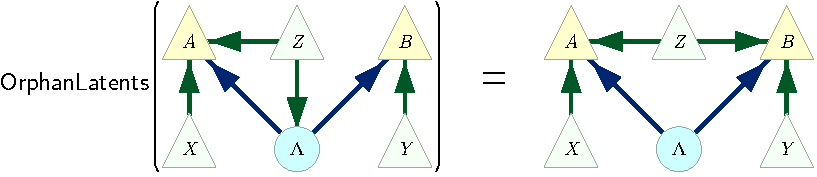
\includegraphics[scale=1]{ExampleOrphanLatents.pdf}
\caption{An example of orphaning latent variables. The latent variable $\Lambda$ had a parent $Z$, so we connected $Z$ directly to $\Lambda$'s children, and disconnected $Z$ from $\Lambda$.}\label{fig:ExampleOrphanLatents}
\end{figure}

\clearpage
\item Add all zero-impact edges from latent variables to their grandchildren, $\mathsf{AdoptGrandchildren}$. This operation adds an edge to the DAG connecting latent variable to one its grandchildren whenever the added edge would leave the DAG observationally invariant. The added edge $\Lambda \to V$ leaves $G$ observationally invariant if $V$ already knows what effect $\Lambda$ has on its descendants. $\Lambda$'s effect is known to $V$ if, given the parents of $V$, the \emph{mutual information} between $\Lambda$'s children and their parents-aside-from-$\Lambda$ is zero, $I\parens*{\NamedFunction{ch}{\!\Lambda\!}:\parens*{\NamedFunction{pa}{\!\NamedFunction{ch}{\!\Lambda\!}\!}/\Lambda}|\NamedFunction{pa}{\!V\!}}=0$. Formally, we add the edge $\Lambda \to V$ if both
\begin{compactenum}
\item  $V$ is already a direct child of every child of $\Lambda$ : $\NamedFunction{ch}{\!\Lambda\!} \subseteq \NamedFunction{pa}{\!V\!}$.
\item  $V$ is already a direct child of every one of $\Lambda$'s co-parents: $\NamedFunction{pa}{\!\NamedFunction{ch}{\!\Lambda\!}\!}/\Lambda \subseteq \NamedFunction{pa}{\!V\!}$.
\end{compactenum}
See \cref{fig:ExampleAdoptGrandchildren} for an example. $\mathsf{AdoptGrandchildren}$ must be recursively applied to a DAG \emph{iteratively}, because sometimes the edge $\Lambda \to V$ OR the edge $\Lambda \to U$ can be added to $G$ without observationally impacting $G$, but both edges cannot be added simultaneously; iterative recursion avoids this concern, see \cref{fig:BadAdoptGrandchildren} for an example. 
%When a single iteration must choose between $\Lambda \to V$ or $\Lambda \to U$ we require $\mathsf{AdoptGrandchildren}$ to use the first instance 
%An examples is $G=\brackets{\Lambda\to A,A\to B,A \to C,Y \to B, Z\to C}$.Second, by applying $\mathsf{AdoptGrandchildren}$ iteratively, one find that sometimes latent variables can adopt great-grandchildren, or even further descendants. 
Transforming a DAG \emph{to the maximum extent possible} via $\mathsf{AdoptGrandchildren}$ leaves the DAG observationally invariant. \purp{Needs better proof.}
\begin{figure}[H]
\centering
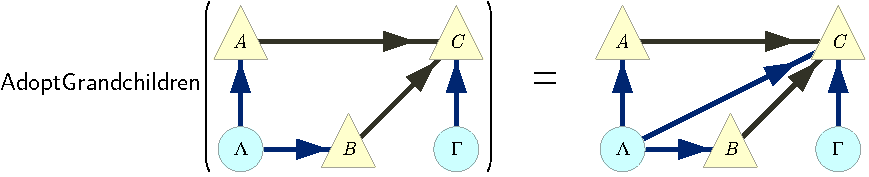
\includegraphics[scale=1]{ExampleAdoptGrandchildren.pdf}
\caption{An example of adopting grandchildren of a latent variable. Here $C$ is a child of both of $\Lambda$'s two children $A$ and $B$. As $A$ and $B$ have no parents other than $\Lambda$ we can add the edge $\Lambda \to C$ without impacting the DAG observationally.}\label{fig:ExampleAdoptGrandchildren}
\end{figure}
\begin{figure}[H]
\centering
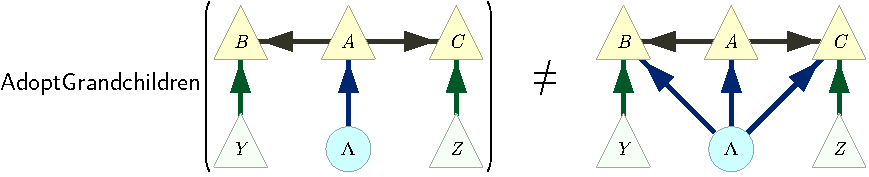
\includegraphics[scale=1]{ExampleNotAdoptGrandchildren.pdf}
\caption{An illustration of why $\mathsf{AdoptGrandchildren}$ must by applied through iterative recursion. Either of the edges $\Lambda \to B$ or $\Lambda \to C$ can be added with zero observational impact, but once one edge is added the addition of the other edge is subsequently precluded.}\label{fig:BadAdoptGrandchildren}
\end{figure}

\item Delete all redundant latent variables, $\mathsf{DeleteRedundantLatents}$. A latent variable $\Lambda$ is redundant is there exists another latent variable $\Gamma$ such that $\Lambda$'s children are a subset of $\Gamma$'s children; if two latent variables have the same children then one of the latent variables is redundant. \purp{Is a proof even required?} This transformation leaves the DAG observationally invariant, see \cref{fig:ExampleDeleteRedundantLatents} for an example.
\begin{figure}[H]
\centering
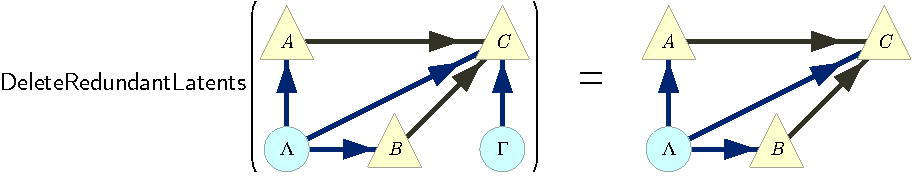
\includegraphics[scale=1]{ExampleDeleteRedundantLatents.pdf}
\caption{An example of deleting redundant latent variables. Here $\Gamma$ is redundant because the randomness in $C$ can be accounted for by $\Lambda$. $\Lambda$'s three children are a strict superset of $\Gamma$'s only child.}\label{fig:ExampleDeleteRedundantLatents}
\end{figure}
\afterpage{\FloatBarrier}

\clearpage
\item Delete all zero-impact edges between ``sibling" variables,  $\mathsf{DisconnectSiblings}$. Siblings are defined as a pair of variables which share at least one common parent. We say that $V$ has perfect knowledge of $U$ if the information flowing to $V$ is enough to ``reconstruct" $U$, i.e. $H \parens{U|\NamedFunction{pa}{\!V\!}}=0$.
If the DAG is expressed in deterministic form (which we assume) then $V$ has perfect knowledge of $U$ whenever $\NamedFunction{pa}{\!U\!} \subseteq \NamedFunction{pa}{\!V\!}$, see Thm. 26.4 and its proof in Ref. \cite{pusey2014gdag}. If $V$ has perfect knowledge of $U$, then the presence or absence of an edge $U \to V$ is observationally irrelevant to the DAG. $\mathsf{DisconnectSiblings}$ seeks out all such edges and deletes them, a transformation which leaves the DAG observationally invariant; see \cref{fig:ExampleDisconnectSibling} for an example.
\begin{figure}[H]
\centering
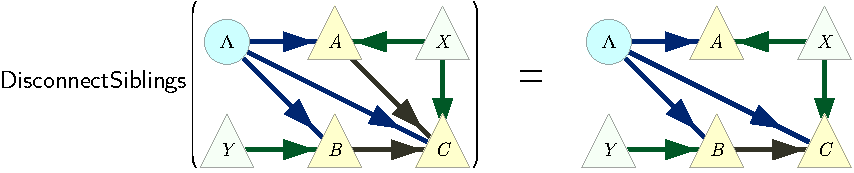
\includegraphics[scale=1]{ExampleDisconnectSibling.pdf}
\caption{An example of removing edges between siblings without observationally impacting the DAG. The edge $A \to C$ can be dropped, as $C$ is a child of all of $A$'a parents, and then some. The edge $B \to C$ \emph{cannot} be removed, however, as $C$ cannot count $Y$ among its parents.}\label{fig:ExampleDisconnectSibling}
\end{figure}

\item Convert a DAG to canonical form, $\mathsf{ToCanonicalForm}$. This just means perform all possible observationally-invariant transformations of the aforementioned kinds to the DAG. The order of operations is as follows: 1) $\mathsf{OrphanLatents}$, 2) $\mathsf{AdoptGrandchildren}$ iterated maximally, 3) $\mathsf{DeleteRedundantLatents}$, 4) $\mathsf{DisconnectSiblings}$. The order of operations is critical. $\mathsf{OrphanLatents}$ shrinks causal pathways, opening up more avenues for $\mathsf{AdoptGrandchildren}$. $\mathsf{AdoptGrandchildren}$ results in variables have new \emph{additional} latent parents, typically meaning some latent variables become redundant. Finally, $\mathsf{DeleteRedundantLatents}$ shrinks the number of parents a given node may have, which opens up more avenues for $\mathsf{DisconnectSiblings}$. In summary,$\NamedFunction{ToCanonicalForm}{G}=
\NamedFunction{DisconnectSiblings}{\NamedFunction{DeleteRedundantLatents}{\NamedFunction{AdoptGrandchildren}{\NamedFunction{OrphanLatents}{G}}}}$, see \cref{fig:ExampleToCanonicalForm} for an example.  $\mathsf{ToCanonicalForm}$ leaves a DAG observationally invariant.  $\mathsf{ToCanonicalForm}$ \emph{presumes} that the input DAG is already in deterministic form, per \cref{fig:ExampleToDeterministic}.
\begin{figure}[H]
\centering
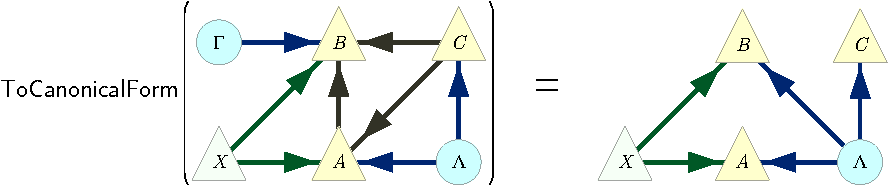
\includegraphics[scale=1]{ExampleToCanonicalForm.pdf}
\caption{An example of transforming a DAG into canonical form. The edge $\Lambda \to B$ is added, which makes $\Gamma$ a redundant latent variable and also gives $B$ incoming connections from 100\% of the parents of $C$, hence we can subsequently remove the $C \to B$ edge.}\label{fig:ExampleToCanonicalForm}
\end{figure}

\begin{prop}\label{prop:CanonicalForm}
%\(\begin{array}{l}
%\text{Two DAGs }G\text{ and }H\text{ are observationally equivalent if and only if}\\
%{\NamedFunction{ToCanonicalForm}{\!G\!}=\NamedFunction{ToCanonicalForm}{\!H\!}}.
%\end{array}\)
\begin{minipage}[t]{0.8\linewidth}
\begin{compactitem}[]
\item Two deterministic-form DAGs $G$ and $H$ are observationally equivalent if \sout{\purp{and only if?}}
 ${\NamedFunction{ToCanonicalForm}{\!G\!}=\NamedFunction{ToCanonicalForm}{\!H\!}}$ .
\end{compactitem}
\end{minipage}
\end{prop}
\begin{proof}The ``if" part is obvious. \purp{``Almost" also ``only if". Sketch: $\mathsf{ToCanonicalForm}$ adds every possible zero-impact edge coming \emph{out of} latent variables are removes every possible zero-impact edge \emph{between} observable variables, while minimizing the number of latent variables. That observational equivalence is not possible with coinciding canonical forms requires multiple sub-proofs: One, the order of operations layed out for $\mathsf{ToCanonicalForm}$ is both necessary and sufficient. Two, \emph{any} transformation other than an element of $\mathsf{ToCanonicalForm}$ \emph{does} have observational impact. The impassable problem, though, is that $\mathsf{AdoptGrandchildren}$ does not always yields a unique DAG, per \cref{fig:BadAdoptGrandchildren}.}\end{proof}

\clearpage
\item Convert all causal pathways into direct causal connections, $\mathsf{AdoptAllDescendants}$. This operation adds edges to the DAG until every root node is directly connected to every one of its causal descendants. This operation generally (but not always) relaxes the DAG observationally\footnote{For causal structures where the correlations between root causes and their eventual effects can never be screened off by some intermediate nodes, such as the scenarios considered in Refs. \cite{fritz2012bell,BeyondBellII}, $\mathsf{AdoptAllDescendants}$ is not a relaxation.}. This is the first step in reducing a DAG to PCC form. Note that all the edges which would be added to a DAG be the operations $\mathsf{OrphanLatents}$ and $\mathsf{AdoptGrandchildren}$ are automatically added under the operation $\mathsf{AdoptAllDescendants}$. Note that latent variables can become redundant under this operation, see \cref{fig:ExampleAdoptDescendants} for an example.
\begin{figure}[H]
\centering
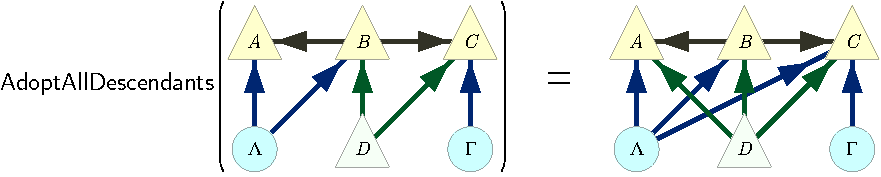
\includegraphics[scale=1]{ExampleAdoptDescendants.pdf}
\caption{An example of converting all causal pathways into direct causal connections. The DAG is relaxed under this transformation, and $\Gamma$ becomes redundant to $\Lambda$.}\label{fig:ExampleAdoptDescendants}
\end{figure}

\item Reduce to purely common cause (PCC) form, $\mathsf{ReduceToPCC}$. This operation is the compound transformation of first applying $\mathsf{AdoptAllDescendants}$ and $\mathsf{DeleteRedundantLatents}$, followed by deleting all edges which don't originate from a root node. Importantly, $\mathsf{ToPCCForm}$ is observationally equivalent to $\mathsf{AdoptAllDescendants}$, despite dropping edges via $\mathsf{ReduceToPCC}$. The proof is intuitive: If $G$ can be interpreted deterministically, then giving a node direct access of all of its \emph{root} ancestors means the node has perfect knowledge about \emph{all} of its ancestors, hence the edges between non-root nodes are of the zero-impact type. Indeed, $\NamedFunction{ReduceToPCC}{G}=\NamedFunction{DisconnectSiblings}{\NamedFunction{DeleteRedundantLatents}{\NamedFunction{AdoptAllDescendants}{G}}}$, see \cref{fig:ExampleToPCC} for an example.
\begin{figure}[H]
\centering
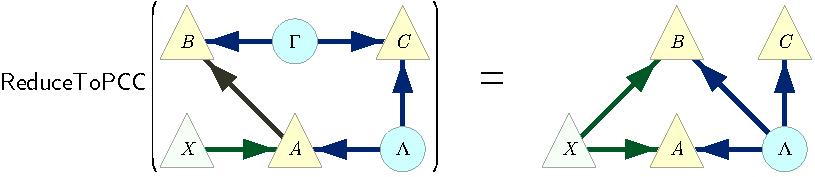
\includegraphics[scale=1]{ExampleToPCC.pdf}
\caption{An example of forcing a DAG into purely common cause (PCC) form. The DAG is relaxed under this transformation. The two edges which are added by $\mathsf{AdoptAllDescendants}$ cannot be justified via $\mathsf{AdoptGrandchildren}$. Note that a latent variable became redundant and was removed during the transformation.}\label{fig:ExampleToPCC}
\end{figure}
\end{itemize}

It should be clear that deterministic-form $G$ and $\NamedFunction{ReduceToPCC}{\!G\!}$ are observationally equivalent if and only if
$G$ and $\NamedFunction{AdoptAllDescendants}{\!G\!}$ are also observationally equivalent. $\NamedFunction{AdoptAllDescendants}{\!G\!}$ is merely $G$ but with (possibly) added edges initiating from $G$'s root nodes. $G$ and $\NamedFunction{AdoptAllDescendants}{\!G\!}$ are therefore observationally equivalent if and only if all the ``new" root edges can be accounted for by observationally invariant transformations. There are, however, \emph{only two} observationally invariable transformations which add \emph{root} edges to a DAG, \sout{both of which only add edges initiating from \emph{latent} variables,} namely $\mathsf{BypassLatents}$ and $\mathsf{AdoptGrandchildren}$. \purp{Proof that no others?} As such,

\begin{prop}
%\(\begin{array}{l}
%\text{Two DAGs }G\text{ and }H\text{ are observationally equivalent if and only if}\\
%{\NamedFunction{ToCanonicalForm}{\!G\!}=\NamedFunction{ToCanonicalForm}{\!H\!}}.
%\end{array}\)
\begin{minipage}[t]{0.8\linewidth}
\begin{compactitem}[]
\item Deterministic-form $G$ and $\NamedFunction{ReduceToPCC}{\!G\!}$ are observationally equivalent if and only if 
%\item
${\NamedFunction{AdoptAllDescendants}{\!G\!}=\NamedFunction{AdoptGrandchildren}{\!\NamedFunction{BypassLatents}{\!G\!}\!}}$.
\end{compactitem}
\end{minipage}
\end{prop}
\begin{comment}
\begin{proof}
By order of operations, $\NamedFunction{ToCanonicalForm}{\!\NamedFunction{ReduceToPCC}{\!G\!}\!}=\NamedFunction{ReduceToPCC}{\!\NamedFunction{OrphanLatents}{\!G\!}\!}$. As such, by \cref{prop:CanonicalForm} we have $G$ and $\NamedFunction{ReduceToPCC}{\!G\!}$ are observationally equivalent if and only \linebreak
${\NamedFunction{ReduceToPCC}{\!\NamedFunction{OrphanLatents}{\!G\!}\!}=\NamedFunction{ToCanonicalForm}{\!G\!}}$. By decomposing both operations it is clear that this equality occurs if and only if $\NamedFunction{AdoptAllDescendants}{\!\NamedFunction{OrphanLatents}{\!G\!}\!}=\NamedFunction{AdoptGrandchildren}{\!\NamedFunction{OrphanLatents}{\!G\!}\!}$, which in turn occurs if and only if $\NamedFunction{AdoptAllDescendants}{\!G\!}=\NamedFunction{AdoptGrandchildren}{\!\NamedFunction{BypassLatents}{\!G\!}\!}$.\end{proof}



\purp{Still writing this new section...}
\end{comment}

\begin{comment}
\section{Triangle Scenario - simple example}\label{sec:TriSimple}


%It is often claimed that classically one must have $\p{a_1 b_1}\geq \p{a_0 b_0}$ from just the first two conditions in  \cref{eq:hardycontrapositive} alone \cite{CabelloHardyInequality}, such that the result ``If additionally $\p{a_1 b_1}=0$ then $\p{a_0 b_0}=0$" is just a special case. 
%We now demonstrate that this Hardy-type inequality follows naturally from assumptions about causal structure. More importantly, we show that Hardy-type arguments can be used to derive compatibility criteria in the same vein even for general causal structures.


\begin{figure*}[t!]
\centering
\subfigure[\hspace{-0.5ex}:\hspace{1ex} The causal structure of the Triangle scenario. Note that there are no direct influences between observable variables.\hfill]
{\begin{minipage}[t]{.45\textwidth}
    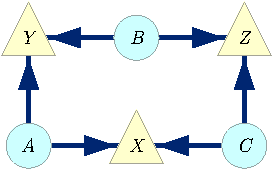
\includegraphics[width=1.8in]{GenuineTriangleDAG.pdf}
    \label{fig:TriDAG}
\end{minipage}}\hfill{\color{gray}\rule[-0.4cm]{0.5pt}{3cm}}\hfill
\subfigure[\hspace{-0.5ex}:\hspace{1ex} An isomorphic directed acyclic graph encoding the causal structure of the Triangle scenario.\hfill]
{\begin{minipage}[t]{.45\textwidth}
    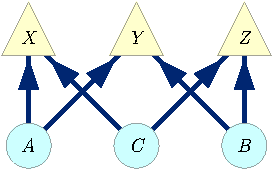
\includegraphics[width=1.8in]{EffectiveTriangleDAG.pdf}
    \label{fig:EffTriDAG}
\end{minipage}}
\vspace{-2ex}\caption{The Triangle scenario: A scenario in which three observable variables are pairwise-correlated but lack a triplewise common ancestor. Conventionally latent variables are indicated by circles while observable variables are indicated by triangles~\cite{pusey2014gdag}.}
\label{fig:Triangle}\vspace{-2ex}
\end{figure*}

%\begin{figure}[b,t]
%\center{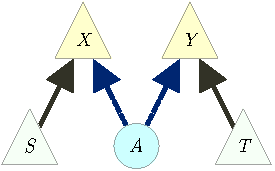
\includegraphics[width=0.7\linewidth]{BellScenarioDAG.pdf}}
%\caption{(color online) The causal structure of the Bell scenario, on which Bell's theorem is based. Per convention, latent variables are indicated by circles whereas observable variables are indicated by triangles \cite{pusey2014gdag}. Observable variables with no incoming edges are setting variables, and are indicated by a light green shading.}
%\label{fig:BellDAG}
%\end{figure}
We first illustrate our method for deriving polynomial inequalities by considering the Triangle scenario [\citealp{pusey2014gdag}~(Fig.~E\#8), \citealp{WoodSpekkens}~(Fig.~18b), \citealp{fritz2012bell}~(Fig.~3), \citealp{chaves2014novel}~(Fig.~6a), \citealp{Chaves2015infoquantum}~(Fig.~1a), \citealp{BilocalCorrelations}~(Fig.~8), \citealp{steudel2010ancestors}~(Fig.~1b), \citealp{chaves2014informationinference}~(Fig.~4b)], the causal structure of which is depicted here in \cref{fig:Triangle}. Here $\brackets{X,Y,Z}$ are the observable variables, and  $\brackets{A,B,C}$ are latent. $A$ denotes the common cause of $X$ and $Y$, etc. The Triangle scenario is a correlation scenario in the sense of \citet{fritz2012bell}; see especially Sec. 2.3 there.

There can be no linear inequality in term of probabilities for the triangle scenario, which makes a polynomial inequality technique especially valuable for this scenario. The nonlinear of the Triangle scenario follows for the non-convexity of the set of all probability distributions which are compatible with it. \purp{Proof of nonconvexity or nonlinearity needed. Tobias?}

Causal structure generally dictates that not all the observable variables depend on all the latent variables, but rather each observable variable depends only in its particular latent ancestors. For the Triangle scenario this means that
\begin{align}\begin{split}\label{eq:tristructure}
%\p{x y z | a b c}=\p{x_{c a}  y_{a b}  z_{b c}}
\p{x_{a b c}}=\p{x_{c a}} \,,\; \p{y_{a b c}}=\p{y_{b c}} \,,\; \p{z_{a b c}}=\p{z_{a b}} \,,\quad\text{and hence}\quad \p{x y z | a b c}=\p{x_{c a}  y_{a b}  z_{b c}}\,,
\end{split}\end{align}
and accordingly, 
\begin{align}\label{eq:triintegration}
&\p{x y z}=\sum\limits_{a\in \norm{A}} \sum\limits_{b\in \norm{B}} \sum\limits_{c\in \norm{C}} \p{x_{c a}  y_{a b}  z_{b c}}\p{a}\p{b}\p{c}.
\end{align}

Here is an example of a quadratic polynomial constraint for the Triangle scenario.
\begin{prop} \label{prop:Deg2}
The Triangle causal structure (\cref{fig:Triangle}) implies that
\begin{align*}
\p{x^1 y^1 z^1} \p{x^2 y^2 z^2}\leq \p{x^1} \p{x^2 y^3}+\p{y^1}\p{x^3 y^2} +\p{z^2}\p{\n{x^3} \n{y^3} z^1} 
\end{align*}
\end{prop}
\begin{proof}
We use the causal structure to consider various counterfactual propositions, which we collect into a logical tautology as follows.
\begin{align}\begin{split}\label{eq:tri2structaut}
&\NamedFunction{And}{ x^1_{c^1 a^1} , y^1_{a^1 b^1} , z^1_{b^1 c^1} , x^2_{c^2 a^2} , y^2_{a^2
   b^2} , z^2_{b^2 c^2} }
 \implies 
\NamedFunction{Or}{
    \NamedFunction{And}{ y^1_{a^1 b^1} , x^3_{c^1 a^2} , y^2_{a^2 b^2} } ,\\
    \NamedFunction{And}{ x^1_{c^1 a^1} , x^2_{c^2 a^2} , y^3_{a^2 b^1} } ,\\
    \NamedFunction{And}{ z^2_{b^2 c^2} , \n{x^3_{c^1 a^2}} , \n{y^3_{a^2 b^1}} , z^1_{b^1 c^1}
   }
}
\end{split}\end{align}
Next, we convert the tautology to an inequality via two rules:
\begin{enumerate}
\item As the antecedent always implies the consequent, the probability of the antecedent is necessarily less-than-or-equal-to the probability of the consequent. If $j \cramp{\scriptstyle \implies} k$ then $\p{j}\leq\p{k}$.
\item The probability of a disjunction of events is less-than-or-equal-to the sum of the probabilities of the individual events, i.e. ${\p{j\lor k}=\p{j}+\p{k}-\p{j,k}\leq \p{j}+\p{k}}$.
\end{enumerate}
The inequality which corresponds to \cref{eq:tri2structaut} is
\begin{align}\begin{split}\label{eq:tri2structineq}
\p{x^1_{c^1 a^1} y^1_{a^1 b^1} z^1_{b^1 c^1}} \p{x^2_{c^2 a^2} y^2_{a^2 b^2} z^2_{b^2 c^2}}\leq \lparens{
  \hphantom{+}\p{x^1_{c^1 a^1}} \p{x^2_{c^2 a^2} y^3_{a^2 b^1}}
\\+\p{y^1_{a^1 b^1}}\p{x^3_{c^1 a^2} y^2_{a^2 b^2}} 
\\+\p{z^2_{b^2 c^2}}\p{\n{x^3_{c^1 a^2}} \n{y^3_{a^2 b^1}} z^1_{b^1 c^1}} }
\end{split}\end{align}
Note that we have factored terms in \cref{eq:tri2structineq} according to distinct counter-factual instances. This is the key step in deriving polynomial inequalities. The distinct counterfactual instances are perhaps best seen by rewriting \cref{eq:tri2structineq} in a manner which does not assume a particular causal structure, namely
\begin{align}\begin{split}\label{eq:tri2operineq}
\p{x^1 y^1 z^1|c^1 a^1 b^1} \p{x^2 y^2 z^2|c^2 a^2 b^2}
\leq
\lparens{
  \hphantom{+}\p{x^1|c^1 a^1} \p{x^2 y^3|c^2 a^2 b^1}
\\+\p{y^1|a^1 b^1} \p{x^3 y^2|c^1 a^2 b^2} 
\\+\p{z^2|b^2 c^2} \p{\n{x^3} \n{y^3} z^1|c^1 a^2 b^1} }
\end{split}\end{align}
which we can marginalize both sides over all  $\brackets{a^1,b^1,c^1,a^2,b^2,c^2}$ to obtain \cref{prop:Deg2}.
\end{proof}
As both \cref{eq:tri2structaut,eq:tri2operineq} can be inferred from \cref{eq:tri2structineq}, we shall include only inequalities written in terms of individual-observable counterfactuals in subsequent proofs of polynomial inequalities.



Note that as a general matter, polynomial inequalities can be relaxed into interesting special cases by \emph{disregarding} some of the negated events. For example, we may suppose that a certain outcome is impossible, for example, we may imagine that $x^3\not\in \norm{X}$ in \cref{prop:Deg2}. We denote this as  $x^3\to \mathsf{False}$. By this substitution we have $\p{\n{x^3} \n{y^3} z^1} \to \p{\n{y^3} z^1}$ and $\p{x^3
   y^2}\to 0$, and thus we obtain the special case
\begin{align}\label{eq:tri2specialcase}
\p{x^1 y^1 z^1} \p{x^2 y^2 z^2}\leq \p{x^1} \p{x^2 y^3}+\p{z^2}\p{\n{y^3} z^1} 
\end{align}
which can be strengthened by ignoring events which do not appear on the right hand side of \cref{eq:tri2specialcase}, namely $\brackets{y^1,y^2}\to \mathsf{True}$.  Thus
\begin{align}
\p{x^1 z^1} \p{x^2 z^2}\leq \p{x^1} \p{x^2 y}+\p{z^2}\p{\n{y} z^1} .
\end{align}
\end{comment}

\begin{comment}
\section{Triangle Scenario - degree 3 example \purp{OLD, new notation needed}}

Here is an example of a cubic polynomial constraint for the Triangle scenario. 
\begin{prop} \label{prop:AllPowerful}
The Triangle causal structure (\cref{fig:Triangle}) implies that
\begin{align*}\begin{split}
\p{x^1 y^1 z^1} \p{x^2 y^2 z^2} \p{x^3 y^3 z^3}
\leq
\lparens{
   \hphantom{+}\p{y^1} \p{x^4 y^3} \p{x^2 y^2 z^2}
\\+\p{z^3} \p{y^4 z^2} \p{x^1 y^1 z^1}
\\+\p{x^2} \p{z^4 x^1} \p{x^3 y^3 z^3}
\\+\p{z^1} \p{x^5 z^2} \p{x^3 y^3 z^3}
\\+\p{x^3} \p{y^5 x^1} \p{x^2 y^2 z^2}
\\+\p{y^2} \p{z^5 y^3} \p{x^1 y^1 z^1}
\\+\p{\n{x^4} \n{y^4} \n{z^4}} \p{\n{x^5} \n{y^5} \n{z^5}}}
\end{split}\end{align*}
\end{prop}
\begin{proof}\cref{prop:AllPowerful} is self-evident from the following inequality
\begin{align}\label{eq:tri3structineq}
\p{x^1_{c^1 a^1} y^1_{a^1 b^1} z^1_{b^1 c^1}} \p{x^2_{c^2 a^2} y^2_{a^2 b^2} z^2_{b^2 c^2}} \p{x^3_{c^3 a^3} y^3_{a^3 b^3} z^3_{b^3 c^3}}
\leq
\lparens{
   \hphantom{+}\p{y^1_{a^1 b^1}} \p{x^4_{c^1 a^3} y^3_{a^3 b^3}} \p{x^2_{c^2 a^2} y^2_{a^2 b^2} z^2_{b^2 c^2}}
\\+\p{z^3_{b^3 c^3}} \p{y^4_{a^3 b^2} z^2_{b^2 c^2}} \p{x^1_{c^1 a^1} y^1_{a^1 b^1} z^1_{b^1 c^1}}
\\+\p{x^2_{c^2 a^2}} \p{z^4_{b^2 c^1} x^1_{c^1 a^1}} \p{x^3_{c^3 a^3} y^3_{a^3 b^3} z^3_{b^3 c^3}}
\\+\p{z^1_{b^1 c^1}} \p{x^5_{c^2 a^1} z^2_{b^2 c^2}} \p{x^3_{c^3 a^3} y^3_{a^3 b^3} z^3_{b^3 c^3}}
\\+\p{x^3_{c^3 a^3}} \p{y^5_{a^1 b^3 x^1_{c^1 a^1}}} \p{x^2_{c^2 a^2} y^2_{a^2 b^2} z^2_{b^2 c^2}}
\\+\p{y^2_{a^2 b^2}} \p{z^5_{b^3 c^2} y^3_{a^3 b^3}} \p{x^1_{c^1 a^1} y^1_{a^1 b^1} z^1_{b^1 c^1}}
\\+\p{\n{x^4_{c^1 a^3}} \n{y^4_{a^3 b^2}} \n{z^4_{b^2 c^1}}} \p{\n{x^5_{c^2 a^1}} \n{y^5_{a^1 b^3}} \n{z^5_{b^3 c^2}}}
}
\qedhere\end{align}
\end{proof}
A special case of \cref{prop:AllPowerful} is
\begin{prop} \label{prop:FritzF2}
The Triangle causal structure (\cref{fig:Triangle}) implies that
\begin{align*}\begin{split}
\p{x}\p{y}\p{z}\leq&   \p{x}\p{y,z} + \p{y}\p{z,x}+ \p{z}\p{x,y}+\p{\n{x},\n{y},\n{z}}.
\end{split}\end{align*}
\end{prop}
\begin{proof}
First, let $\brackets{x^5,y^5,z^5}\to\mathsf{False}$ and $\brackets{x^2,x^3,y^1,y^2,z^1,z^3}\to\mathsf{True}$. This yields
\begin{align}
\p{x^1 } \p{z^2} \p{y^3}
\leq
{\p{x^4 y^3} \p{z^2}
+\p{y^4 z^2} \p{x^1}
+\p{z^4 x^1} \p{y^3}
+\p{\n{x^4} \n{y^4} \n{z^4}}}
\end{align}
which reduces to \cref{prop:FritzF2} by further substituting $x^4\to x^1$, $y^4\to y^3$, and $z^4\to z^2$.
\end{proof}


A consequence of \cref{prop:FritzF2} is that the W-type distribution
\begin{align}\label{eq:wdistribution}
p_{\text{W}}\parens{x,y,z}=\begin{cases}\tfrac{1}{3}&\text{if }\; x+y+z=1 \\ 0&\text{otherwise}\end{cases}
\end{align}
is found to be incompatible with the Triangle scenario, where $x,y,z\in\brackets{0,1}$. The W-distribution states that the in any event in which $X,Y,Z$ are observed, precisely one of them will be found to equal $1$ while the other two will equal $0$. The identity of the variable which takes the value $1$ is uniformly random. In informal but intuitive notation, the W-type distribution is ${\nicefrac{1}{3}[100]+\nicefrac{1}{3}[010]+\nicefrac{1}{3}[001]}$.
To see how this distribution is incompatible with \cref{prop:FritzF2}, note that for three \emph{identically distributed} (but not independent) binary variables a further special case of \cref{prop:FritzF2} is
\begin{align*}\begin{split}
&\hspace{-6ex}\p{X\cramp{=}1}^3\leq \p{X\cramp{=}Y\cramp{=}Z\cramp{=}0} + 3\times\p{X\cramp{=}1,Y\cramp{=}1}\p{Z\cramp{=}1}.
\end{split}\end{align*}
For the W-distribution ${\p{X\cramp{=}Y\cramp{=}Z\cramp{=}0}=0}$, and also ${\p{X\cramp{=}1,Y\cramp{=}1}=0}$, yet ${\p{X\cramp{=}1}=\nicefrac{1}{3}}$. As ${(\nicefrac{1}{3})^3\nleq 0}$ we have proven that the W-type distribution is incompatible with the Triangle scenario.
\end{comment}



\begin{comment}
\section{Latent Reduction \purp{NEW SECTION AS OF NOV 5.}}\label{sec:LR}
\purp{Everything about latent reduction is now consolidated here. Maybe use the S20 DAG (\cref{fig:S20Scenario}) as an example?}

In everything that follows we consider exclusively \tred{latent completed} causal structures. A latent completed causal structure is one in which \sout{all root vertices are latent} every observable has at least one latent parent. A latent incomplete structure can be completed without loss of generality by supplementing it with latent variables as necessary. For any root note that isn't latent we simply add to it a unique latent parent. \purp{Worth having a figure?} 
We denote the set of observable probability distributions compatible with a causal structure $G$ by $\mathcal{C}_G$. $\mathcal{C}_G$ is invariant under latent completion.

The operation of latent reduction has two steps:

\begin{compactenum}
\item Modify $G$ by directly connecting each latent variable to every observable variable which is in its causal future.\\ ${\Lambda \leadsto V \text{ becomes } \Lambda \to V \text{ whenever } \Lambda\in \NamedFunction{LatentVars}{\!G\!}}$.
\item Modify $G$ further by deleting all edges connecting pairs of observable variable.\\ ${U \to V \text{ becomes } U \not\to V \text{ whenever } U\not\in \NamedFunction{LatentVars}{\!G\!}}$.
\end{compactenum}


It isn't hard to show that latent reduction is a relaxation of the causal structure, and hence $\mathcal{C}_G \subseteq \mathcal{C}_{G'}$. 

Because every observable variable is a child of a latent variable we may take all functional dependencies between variables to be deterministic without loss of generality [\citealp[Conj.~4.5]{BeyondBellII}, see also \citealp{FineTheorem}, \citealp{SpekkensDeterminism}, and \citealp[Rmk.~2.3]{fritz2012bell}]. 
In other words, every variable may be presumed to be an \emph{injective function} of its parents. Since the root nodes of $G$ are all latent variables, we may treat each observable as an explicit function of its latent ancestors without loss of generality \citep[Sec.~4]{lee2015causalinference}. The bottom line is this: \tred{$G'$ is generally a relaxation of $G$; any causal compatibility criteria applicable to $G'$ is therefore also applicable to $G$.}

Latent reductions will always yield bipartite graphs, connecting one layer of latent variables to another layer of observable variables. A latent reduction can also be represented via a hypergraph \citep[Def.~3.2]{fritz2012bell}. 

Mapping genuine causal structures into their latent reductions has previously been recognized as an effective technique in causal inference, see Refs. \citep[Thm. 2.4]{fritz2012bell} and \citep[Sec. 5]{BilocalCorrelations}. Our inequalities apply to the latent reductions, and hence only indirectly to their generating causal structures. Causal structures which are isomorphic to their latent reductions, including the Triangle scenario, have been studied at length by \citet{fritz2012bell}; the connection to more general causal structures is further elucidated in Ref. \cite{BeyondBellII}. Latent-reduced causal structures are also known as ``correlation scenarios" \cite{fritz2012bell} or ``purely common cause" scenarios \cite{lee2015causalinference}.


Different causal structures can have the same latent reduction, in which case the inequalities we derive will not be able to distinguish such structure, for example $G\neq \NamedFunction{LR}{\!G\!}\neq H$, but $\NamedFunction{LR}{\!G\!}= \NamedFunction{LR}{\!\NamedFunction{LR}{\!G\!}\!}= \NamedFunction{LR}{\!H\!}$. If two structure have the same latent reduction we call them \tred{equivalent under latent reduction}.

Causal compatibility criteria on $G'$ are also necessary constraints on $G$ by virtue of $\mathcal{C}_G \subseteq \mathcal{C}_{G'}$. When  $\mathcal{C}_G = \mathcal{C}_{G'}$, i.e. when latent reduction does not actually relax the set of compatible observable probability distributions, we call $G$ \tred{lossless under latent reduction}.  ``Correlation scenarios" \cite{fritz2012bell} are isomorphic to their latent reductions, and hence are trivially lossless under latent reduction. 

Quantum physicists may which to note the following result \citep[Thm.~3.8]{fritz2012bell}: Correlation scenarios which are star graphs \citep[Fig.~6]{fritz2012bell} do not admit uniquely-quantum (non-classical) probability distributions. That is, replacing classical latent variables with quantum states does not expand the set of possible observable distributions beyond $C_G$ for such correlation structures. Consequently, all general causal structures which are star graphs under latent reduction also do not admit quantum probability distributions. The classification of causal structures which admit non-classical probability distributions has been addressed in further detail by \citet{pusey2014gdag}. 

Causal structures which are lossless under latent reduction are happily plentiful in quantum foundations; in particular, all $k$-partite Bell scenarios have been proven to be lossless under latent reduction \citep[Thm.~2.24]{fritz2012bell}! As such, our the inequalities we can derive have maximum restrictive power for $k$-partite Bell scenarios.

If there is a ${\Lambda\in \NamedFunction{LatentVars}{\!G'\!}}$ which is a parent of every observable variable in $G'$, then $\mathcal{C}_{G'}$ is totally unrestricted \citep[Prop.~3.7]{fritz2012bell}. Such $G'$ arise whenever there exists ${\Lambda\in \NamedFunction{LatentVars}{\!G\!}}$ which is \emph{ancestral} to all of the observable variables in $G$. Our technique cannot derive non-trivial inequalities for such scenarios. Such scenarios include the Instrumental scenario \cite{pearl2009causality,spirtes2011causation,studeny2005probabilistic,koller2009probabilistic} (when latent completed), and the Unrelated Confounding scenario \cite{evans2012graphical}, for examples. 

$G$ is certainly lossy under latent reduction if $G$ has conditional independence relations which are absent in $G$. Latent reduction scenario can only have \emph{unconditional} independence relations, so if $G$ has any \emph{conditional} independence relation then $G$ is lossy under latent reduction. \purp{Suggests different bi-partitioning of causes and effects?}



\section{Observational Equivalence of Non-Isomorphic DAGs \purp{NEW SECTION AS OF NOV 11.}}\label{sec:OE}

Adding an edge $\Lambda \to V$ does not change $\mathcal{C}_{G}$ if both the following two conditions are both met: 

1) $V$ is already a direct child of every child of $\Lambda$ : $\NamedFunction{ch}{\!\Lambda\!} \subseteq \NamedFunction{pa}{\!V\!}$.

2) $V$ is already a direct child of every one of $\Lambda$'s co-parents: $\NamedFunction{pa}{\!\NamedFunction{ch}{\!\Lambda\!}\!}/\Lambda \subseteq \NamedFunction{pa}{\!V\!}$.

\noindent If these conditions are met then $V$ already knows what effect $\Lambda$ has on its descendants, so providing $V$ direct access to the information of  $\Lambda$ does not strengthen any correlation.

Adding an edge $X \to Y$ does not change $\mathcal{C}_{G}$ if the following condition is met: 

1) $Y$ is already a direct child of every parent of $X$ : $\NamedFunction{pa}{\!X\!} \subseteq \NamedFunction{pa}{\!Y\!}$.

\noindent Treating the each variable as a deterministic injective function of its parents means that the variables serving as input to $Y$ are sufficient to reconstruct the function $X$, so providing $Y$ direct access to the information of $X$ does not strengthen any correlation.

Adding edges to $G$ pursuant to these conditions allow us to determine if $G$ is certainly lossy under latent reduction.






\section{Bell Scenario}
\begin{figure*}[t!]
\centering
\subfigure[\hspace{-0.5ex}:\hspace{1ex} The causal structure of the Bell scenario. Conventionally $S$ and $T$ are considered experimental settings; we depict the \tred{latent completed} structure, in which we imagine the settings are selected according to some local hidden variables.\hfill]
{\begin{minipage}[t]{.45\textwidth}
    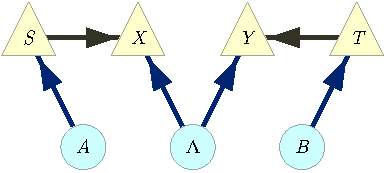
\includegraphics[width=2.55in]{GenuineBellDAG.pdf}
    \label{fig:BellDAG}
\end{minipage}}\hfill{\color{gray}\rule[-0.4cm]{0.5pt}{3cm}}\hfill
\subfigure[\hspace{-0.5ex}:\hspace{1ex} The \tred{latent reduction} of the Bell scenario. Influences between observables have been deleted, but every observable is now directly connected to all of its latent ancestors. See Fig.~1 in Ref. \cite{fritz2012bell}. \hfill]
{\begin{minipage}[t]{.45\textwidth}
    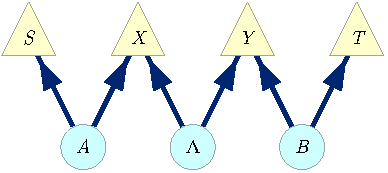
\includegraphics[width=2.55in]{EffectiveBellDAG.pdf}
    \label{fig:EffBellDAG}
\end{minipage}}
\vspace{-2ex}\caption{The Bell scenario: A scenario in which ${X}\cramp{\perp}{T}$ and ${Y}\cramp{\perp}{S}$ but ${X}\cramp{\not\perp}{Y}$. The Bell scenario is particularly famous in quantum theory \cite{bell1966lhvm,Brunner2013Bell,WoodSpekkens}, as many non-local correlations have be generated by replacing $\Lambda$ with some quantum $\bm\rho$.}
\label{fig:Bell}\vspace{-2ex}
\end{figure*}

Consider the causal structure associated to the Bell/CHSH \cite{bell1964einstein,Brunner2013Bell,bell1966lhvm,CHSHOriginal} experiment [\citealp{pusey2014gdag}~(Fig.~E\#2), \citealp{WoodSpekkens}~(Fig.~19), \citealp{chaves2014novel}~(Fig.~1), \citealp{BeyondBellII}~(Fig.~1), \citealp{wolfe2015nonconvexity}~(Fig.~2b), \citealp{steeg2011relaxation}~(Fig.~2)], depicted here in \cref{fig:BellDAG}. $\brackets{S,T,X,Y}$ are all observable variables and $\Lambda$ is the latent common cause of $X$ and $Y$.

%Without loss of generality let's assume that the values $\Lambda\mathopen{=}\lambda$ are drawn from some (possibly infinite, possibly continuous) set $\lambda\in\Omega$. 
The assumption of causal structure dictates that
\begin{align}\begin{split}\label{eq:bellstructure}
%\p{x y s t | \lambda a b}=\p{x_{\lambda a} y_{\lambda b} s_x t_y}
\p{x_{\lambda a b}}=\p{x_{\lambda a}} \,,\; \p{y_{\lambda a b}}=\p{y_{\lambda b}} \,,\; \p{s_{\lambda a b}}=\p{s_{a}} \,,\; \p{t_{\lambda a b}}=\p{t_{b}} \,,%\quad\text{and hence}\quad \p{x y s t | \lambda a b}=\p{x_{\lambda a} y_{\lambda b} s_x t_y}\,,
%=\p{x_{s|\lambda}}\p{y_{t|\lambda}}
\end{split}\end{align}
and hence
\begin{align}\begin{split}\label{eq:bellintegration}
&\p{x y s t | \lambda a b}=\p{x_{\lambda a} y_{\lambda b} s_a t_b}\,,\quad\text{and accordingly}\quad \p{x y s t}=\sum\limits_{{\lambda\in \norm{\Lambda}}}\sum\limits_{{a\in \norm{A}}}\sum\limits_{{b\in \norm{B}}}\p{x_{\lambda a} y_{\lambda b} s_a t_b}\p{\lambda}\p{a}\p{b}.
\end{split}\end{align}
These ancestral-latent dependencies per \cref{eq:bellstructure} are used to map the genuine Bell causal structure (\cref{fig:BellDAG}) to its latent reduction, namely \cref{fig:EffBellDAG}, which \tred{implies the same latent independencies}. The Bell causal structure is known to be lossless under latent reduction \citep[Thm.~2.4]{fritz2012bell}, so \cref{fig:BellDAG} and \cref{fig:EffBellDAG} are indeed observationally equivalent.

An important causal criterion is as follows. 
\begin{prop} \label{prop:CH}
The Bell causal structure (\cref{fig:Bell}) implies that
\begin{align*}
\p{x^1 y^1 s^1 t^1} \p{x^2 y^2 s^2 t^2}
\leq
\p{x^2 s^2 t^1} \p{x^1 y^3 s^1 t^2}
+\p{y^2 s^1 t^2} \p{x^3 y^1 s^2 t^1}
+\p{s^1 t^1} \p{\n{x^3} \n{y^3} s^2 t^2}
\end{align*}
\end{prop}

\begin{proof}
To prove \cref{prop:CH}, start with this logical tautology pursuant to \cref{fig:EffBellDAG}
\begin{align}\begin{split}
\NamedFunction{And}{ x^1_{\lambda ^1 a^1} , y^1_{\lambda ^1 b^1} , s^1_{a^1} , t^1_{b^1} , x^2_{\lambda ^2 a^2} , y^2_{\lambda ^2 b^2} , s^2_{a^2} , t^2_{b^2} }
\implies 
\NamedFunction{Or}{
    \NamedFunction{And}{ x^2_{\lambda ^2 a^2} , s^2_{a^2} , t^1_{b^1} , x^1_{\lambda ^1 a^1} , y^3_{\lambda ^1 b^2} , s^1_{a^1} , t^2_{b^2} } ,\\
    \NamedFunction{And}{ y^2_{\lambda ^2 b^2} , s^1_{a^1} , t^2_{b^2} , x^3_{\lambda ^1 a^2} , y^1_{\lambda ^1 b^1} , s^2_{a^2} , t^1_{b^1} } ,\\
    \NamedFunction{And}{ s^1_{a^1} , t^1_{b^1} , \n{x^3_{\lambda ^1 a^2}} , \n{y^3_{\lambda ^1 b^2}} , s^2_{a^2} , t^2_{b^2} } 
}
\end{split}\end{align}
which converts to the inequality
\begin{align}\begin{split}\label{eq:bellstructineq}
\p{x^1_{\lambda ^1 a^1} y^1_{\lambda ^1 b^1} s^1_{a^1} t^1_{b^1}} \p{x^2_{\lambda ^2 a^2} y^2_{\lambda ^2 b^2} s^2_{a^2} t^2_{b^2}}
\leq
\lparens{
\hphantom{+}\p{x^2_{\lambda ^2 a^2} s^2_{a^2} t^1_{b^1}} \p{x^1_{\lambda ^1 a^1} y^3_{\lambda ^1 b^2} s^1_{a^1} t^2_{b^2}}
\\+\p{y^2_{\lambda ^2 b^2} s^1_{a^1} t^2_{b^2}} \p{x^3_{\lambda ^1 a^2} y^1_{\lambda ^1 b^1} s^2_{a^2} t^1_{b^1}}
\\+\p{s^1_{a^1} t^1_{b^1}} \p{\n{x^3_{\lambda ^1 a^2}} \n{y^3_{\lambda ^1 b^2}} s^2_{a^2} t^2_{b^2}}
}
\end{split}\end{align}
or, equivalently,
\begin{align}
\p{x^1 y^1 s^1 t^1|\lambda ^1 a^1 b^1} \p{x^2 y^2 s^2 t^2|\lambda ^2 a^2 b^2}
\leq
\lparens{
\hphantom{+}\p{x^2 s^2 t^1|\lambda ^2 a^2 b^1} \p{x^1 y^3 s^1 t^2|\lambda ^1 a^1 b^2}
\\+\p{y^2 s^1 t^2|\lambda ^2 b^2 a^1} \p{x^3 y^1 s^2 t^1|\lambda ^1 a^2 b^1}
\\+\p{s^1 t^1|a^1 b^1} \p{\n{x^3} \n{y^3} s^2 t^2|\lambda ^1 a^2 b^2}
}\,.
\end{align}
To complete the proof we simply marginalize both sides over $\brackets{\lambda ^1, a^1, b^1,\lambda ^2, a^2, b^2}$.\end{proof}


A special case of \cref{prop:CH} is obtained by setting $\brackets{x^2,y^2}\to\mathsf{True}$, $x^3\to \n{x^1}$, and $y^3\to \n{y^1}$. This yields
\begin{align}
\p{x y s^1 t^1} \p{s^2 t^2}
\leq
\p{s^2 t^1} \p{x \n{y} s^1 t^2}
+\p{s^1 t^2} \p{\n{x} y s^2 t^1}
+\p{s^1 t^1} \p{x y s^2 t^2}
\end{align}
which is better understood in conditional form, namely
\begin{align}
\p{x y | s^1 t^1} \p{s^1 t^1}\p{s^2 t^2}
\leq
\p{x \n{y} | s^1 t^2}\p{s^1 t^2}\p{s^2 t^1} 
+\p{\n{x} y | s^2 t^1}\p{s^2 t^1}\p{s^1 t^2} 
+\p{x y | s^2 t^2}\p{s^2 t^2}\p{s^1 t^1}.
\end{align}
However, the Bell scenario causal structure further implies that $\p{s t}=\p{s}\p{t}$, and hence
\begin{align}
\p{x y | s^1 t^1}
\leq
\p{x \n{y} | s^1 t^2}
+\p{\n{x} y | s^2 t^1}
+\p{x y | s^2 t^2}.
\end{align}
Finally, we may eliminate negation notation entirely by substituting $\p{x \n{y} | s t} \to \p{x | s t}-\p{x y | s t} = \p{x | s}-\p{x y | s t}$ etc. Thus we obtain
\begin{align}
\p{x y | s^1 t^1} + \p{x y | s^1 t^2} + \p{x y | s^2 t^1}
\leq
\p{x | s^1}
+\p{y | t^1}
+\p{x y | s^2 t^2}.
\end{align}
which is simply the Clauser-Horne (CH) inequality \cite{CHInequality} for the Bell scenario. The CH inequality is the \emph{unique} Bell inequality (up to permutations) for the Bell scenario if $\brackets{S,T,X,Y}$ are all binary, and hence the CH inequality is a necessary and sufficient criterion to ascertain if correlations are compatible with that Bell scenario variant.


\end{comment}

















\begin{comment}
\clearpage
\section{Other Causal Scenarios}
Here we present a few other causal structures of note and some polynomial inequalities which are justified by our method. Many more inequalities for these scenarios, and also additional scenarios, \purp{will be} considered in the Supplementary Materials.
\begin{figure*}
\centering
\subfigure[\hspace{-0.5ex}:\hspace{1ex} The causal structure of the S15 scenario. Implies ${Z}\cramp{\perp}{W}$. ${X}\cramp{\perp}{Y}|W$ is also implied if the dotted edges $A\to X$ and $A\to Y$ are absent. \hfill]
{\begin{minipage}[t]{.45\textwidth}
    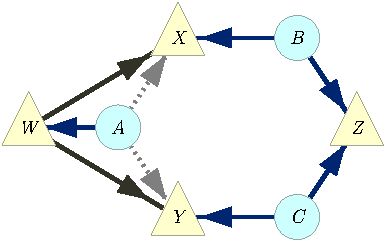
\includegraphics[width=2.55in]{GenuineS15DAG.pdf}
    \label{fig:S15DAG}
\end{minipage}}
\hfill{\color{gray}\rule[-0.4cm]{0.5pt}{3cm}}\hfill
%\hfill{\color{gray}\rule[-0.4cm]{0.5pt}{3cm}}$\quad\longmapsto\quad${\color{gray}\rule[-0.4cm]{0.5pt}{3cm}}\hfill
\subfigure[\hspace{-0.5ex}:\hspace{1ex} The latent reduction of the S15 scenario. Implies only ${Z}\cramp{\perp}{W}$. \hfill]
{\begin{minipage}[t]{.45\textwidth}
    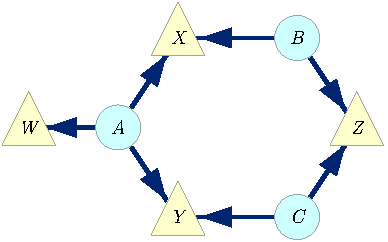
\includegraphics[width=2.55in]{EffectiveS15DAG.pdf}
    \label{fig:EffS15DAG}
\end{minipage}}
\vspace{-2ex}\caption{\purp{Two variants of the S15 scenario, so named because the ``empty" variant is listed as ``interesting" structure \#15 in Ref. \cite[Appx. E]{pusey2014gdag}. The ``empty" variant excludes the dotted edges, the ``full" variant includes them. The empty variant is lossy under latent reduction, but the full variant is lossless. Both variants have the same latent reduction.}\hfill
\\{\color{gray}\rule{\textwidth}{0.5pt}}
}
\label{fig:S15Scenario}\vspace{-3ex}
\end{figure*}




\begin{figure*}
\centering
\subfigure[\hspace{-0.5ex}:\hspace{1ex} The causal structure of the S20 scenario. Implies ${Z}\cramp{\perp}{W}$. ${Y}\cramp{\perp}{W}|X$ is also implied if the dotted edges $Z\to Y$ and $W\to Y$ are absent. \hfill]
{\begin{minipage}[t]{.45\textwidth}
    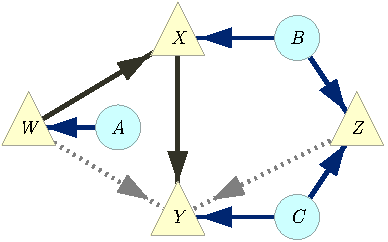
\includegraphics[width=2.55in]{GenuineS20DAG.pdf}
    \label{fig:S20DAG}
\end{minipage}}
\hfill{\color{gray}\rule[-0.4cm]{0.5pt}{3cm}}\hfill
%\hfill{\color{gray}\rule[-0.4cm]{0.5pt}{3cm}}$\quad\longmapsto\quad${\color{gray}\rule[-0.4cm]{0.5pt}{3cm}}\hfill
\subfigure[\hspace{-0.5ex}:\hspace{1ex} The latent reduction of the S20 scenario. Implies only ${Z}\cramp{\perp}{W}$.\hfill]
{\begin{minipage}[t]{.45\textwidth}
    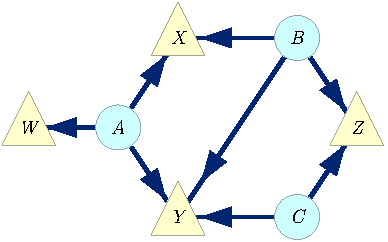
\includegraphics[width=2.55in]{EffectiveS20DAG.pdf}
    \label{fig:EffS20DAG}
\end{minipage}}
\vspace{-2ex}\caption{\purp{Two variants of the S20 scenario, so named because the ``empty" variant is listed as ``interesting" structure \#20 in Ref. \cite[Appx. E]{pusey2014gdag}. The ``empty" variant excludes the dotted edges, the ``full" variant includes them. The empty variant is lossy under latent reduction, but the full variant is lossless. Both variants have the same latent reduction.}\hfill
\\{\color{gray}\rule{\textwidth}{0.5pt}}
}
\label{fig:S20Scenario}\vspace{-3ex}
\end{figure*}


\begin{figure*}
\centering
\subfigure[\hspace{-0.5ex}:\hspace{1ex} The causal structure of the S7 scenario. Implies ${Z}\cramp{\perp}{W}$.\hfill]
{\begin{minipage}[t]{.45\textwidth}
    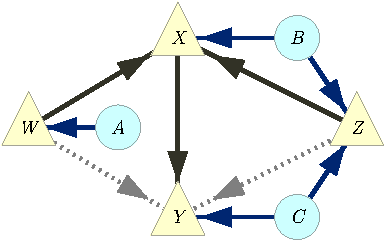
\includegraphics[width=2.55in]{GenuineS7DAG.pdf}
    \label{fig:S7DAG}
\end{minipage}}
\hfill{\color{gray}\rule[-0.4cm]{0.5pt}{3cm}}\hfill
%\hfill{\color{gray}\rule[-0.4cm]{0.5pt}{3cm}}$\quad\longmapsto\quad${\color{gray}\rule[-0.4cm]{0.5pt}{3cm}}\hfill
\subfigure[\hspace{-0.5ex}:\hspace{1ex} The latent reduction of the S7 scenario. Implies ${Z}\cramp{\perp}{W}$.\hfill]
{\begin{minipage}[t]{.45\textwidth}
    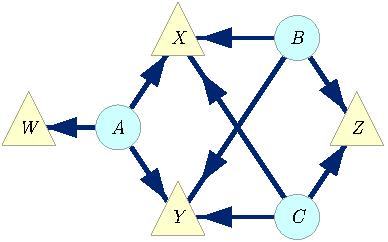
\includegraphics[width=2.55in]{EffectiveS7DAG.pdf}
    \label{fig:EffS7DAG}
\end{minipage}}
\vspace{-2ex}\caption{\purp{Two variants of the S7 scenario, so named because the ``empty" variant is listed as ``interesting" structure \#7 in Ref. \cite[Appx. E]{pusey2014gdag}. The ``empty" variant excludes the dotted edges, the ``full" variant includes them. Both variants are lossy under latent reduction; both variants have the same latent reduction.}\hfill
}
\label{fig:S7Scenario}\vspace{-2ex}
\end{figure*}


\begin{prop}\label{prop:S15deg2example}
The S7 causal structure (\cref{fig:S7Scenario}) implies that
\begin{align*}
&\p{w^1} \p{w^2} \p{x y z^1 w^3}
\leq
{
\p{w^2} \p{z^2 w^1} \p{x y z^1 w^3}
+\p{w^1} \p{\n{z^2} w^2} \p{x y z^1 w^3}
}\,.
%\end{align*}
%\begin{align*}
\\\hspace{-\mathindent}\textit{Proof.}\qquad &\p{w^1_{a^1}} \p{w^2_{a^3}} \p{x_{a^2 b^2 c^2} y_{a^2 b^2 c^2} z^1_{b^2 c^2} w^3_{a^2}}
\leq
\lparens{
\hphantom{+}\p{w^2_{a^3}} \p{z^2_{b^1 c^3} w^1_{a^1}} \p{x_{a^2 b^2 c^2} y_{a^2 b^2 c^2} z^1_{b^2 c^2} w^3_{a^2}}
\\+\p{w^1_{a^1}} \p{\n{z^2_{b^1 c^3}} w^2_{a^3}} \p{x_{a^2 b^2 c^2} y_{a^2 b^2 c^2} z^1_{b^2 c^2} w^3_{a^2}}
}\,.
\end{align*}
\end{prop}
\end{comment}

\clearpage
\begin{acknowledgments}
%\bigskip\noindent\textbf{Acknowledgments}
Research at Perimeter Institute is supported by the Government of Canada through Industry Canada and by the Province of Ontario through the Ministry of Economic Development and Innovation.
\end{acknowledgments}

%\section*{References}
%\nocite{*}
%\setlength{\bibsep}{\smallskipamount}
\setlength{\bibsep}{3pt plus 3pt minus 2pt}
\bibliographystyle{apsrev4-1}
\nocite{apsrev41Control}
\bibliography{apsrevcontrol,hardyinference}


\onecolumngrid
\appendix
\renewcommand{\theequation}{A-\arabic{equation}}
\setcounter{equation}{0}


%%%%%%%%%%%% Enumeration via lowercase letters
\renewcommand{\labelenumi}{(\alph{enumi})}
\renewcommand{\theenumi}{(\alph{enumi})}
\renewcommand{\labelitemi}{$\circ$}

\begin{comment}
\section{Alternative Purely Common Cause DAGs}
\begin{figure}[h]
\centering
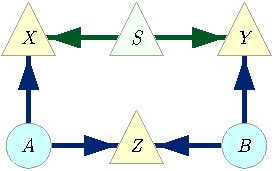
\includegraphics[width=1.82in]{GenuineS15DAGshort.pdf}
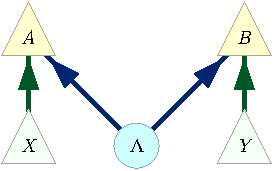
\includegraphics[width=1.82in]{NewBellDAG.pdf}
\caption{The S15 scenario of \cref{fig:S15DAG} and the Bell scenario of \cref{fig:BellDAG}, redrawn so as to be automatically in PCC form, and hence lossless under these ALTERNATIVE PCC reductions.}
\end{figure}



\begin{figure}[h]
\centering
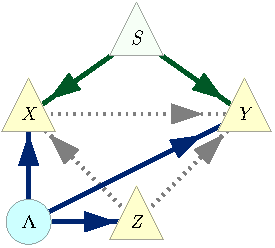
\includegraphics[width=1.82in]{d20eff.pdf}
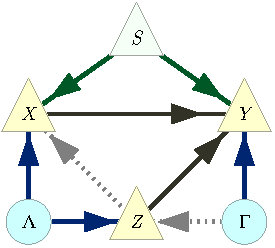
\includegraphics[width=1.82in]{d20alt.pdf}
\caption{By adding or removing the dashed edges, these 2 figures represent 8+4 distinct DAGs. All 12 are observationally equivalent. The PCC reduction of all 12 is the left-side DAG with no dashed edges, therefore all 12 DAGs are lossless under PCC reduction.}\label{fig:e20}
\end{figure}

\begin{figure}[h]
\centering
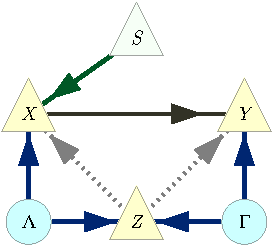
\includegraphics[width=1.82in]{notequiv.pdf}
\caption{By adding or removing the dashed edges, this represent 4 distinct DAGs. All 4 are observationally DISTINCT from each-other, and from the DAGs in \cref{fig:e20}. However the  PCC reduction of all 4 the same, namely the left-side DAG in \cref{fig:e20} with no dashed edges. As such, all 4 DAGs here are LOSSY under PCC reduction.}
\end{figure}

\clearpage
\end{comment}

\section{Tobias's Original 7 Inequalities}

``I present several inequalities... together with a method of proof which has a combinatorial flavour. No quantum violations of any of these inequalities has been found to date.

In the following the complement of a value is marked by an empty circle accent, so $\mathring{b}$ means ``anything but $b$", and accordingly $P(\mathring{a}\mathring{b})=P(A\mathopen{\neq}a,B\mathopen{\neq}b)$. 
%Additionally, an underscore stands for the corresponding marginal probability, like this: $P(\_b\_) := P(abc) + P(ab\mathring{c}) + P(\mathring{a}bc) + P(\mathring{a}b\mathring{c})$. 
\begin{theorem}
The following inequalities hold for all classical correlations in the triangle scenario:
\begin{enumerate}
\item
\(\quad
%--(a)--
%P(0\_\_)P(\_\_1) \leq P(00\_)+P(\_11)
P(a) P(c)  \leq  P(a b) + P(\nb c)
\)
\item
\(\quad
%--(b)--
%P(001) P(010) P(100)  \leq  P(000) + P(11\_) P(001) P(0\_\_) + P(1\_1) P(010) P(\_\_0) + P(\_11) P(100) P(\_0\_)
P(a b\nc) P(a \nb c) P(\na b c) \leq P(a b c) + P(\na \nb) P(a b \nc) P(a) + P(\na\nc) P(a\nb c) P(c)  + P(\nb \nc) P(\na b c) P(b)
\)
\item 
\(\quad
%--(c)--
%P(001) P(010) P(100) \leq  P(000)^2 + 2 P(11\_) P(001) + 2 P(1\_1) P(010) + 2 P(\_11) P(100)
P(a b\nc) P(a \nb c) P(\na b c) \leq P(a b c)^2 + 2\parens*{P(\na \nb) P(a b \nc) + P(\na\nc) P(a\nb c)  + P(\nb \nc) P(\na b c)}
\)
\item
\(\quad
%--(d)--
%P(000)^2 P(111)  \leq  P(001) P(010) P(100) + (2 P(000) + P(111)) (1 - P(000) - P(111))
P(a b c)^2 P(\na\nb\nc)  \leq  P(a b \nc) P(a \nb c) P(\na b c) + \parens*{2 P(a b c) + P(\na\nb\nc)} \parens*{1 - P(a b c) - P(\na\nb\nc)}
\)
\item
\(\quad
%--(e)--
%P(000)^2 P(111)  \leq  P(000)^3 + (2 P(000) + P(111)) (1 - P(000) - P(111))
P(a b c)^2 P(\na\nb\nc)  \leq  P(a b c)^3 + \parens*{2 P(a b c) + P(\na\nb\nc)} \parens*{1 - P(a b c) - P(\na\nb\nc)}
\)
\item
\(\quad
%--(f)--
%P(1\_\_)P(\_1\_)P(\_\_1) \leq P(000)+P(11\_)P(\_\_1)+P(1\_1)P(\_1\_)+P(\_11)P(1\_\_)
P(a) P(b) P(c) \leq  P(\na\nb\nc) + P(a b) P(c) + P(a c) P(b) + P(b c) P(a)
\)
\item
\(\quad
%--(g)--
%P(1\_\_)P(\_1\_)P(\_\_1) \leq P(000)^2+2 P(11\_)P(\_\_1) + 2 P(1\_1)P(\_1\_) + 2 P(\_11)P(1\_\_)
P(a) P(b) P(c) \leq  P(\na\nb\nc)^2 +2\parens[\Big]{ P(a b) P(c) + P(a c) P(b) + P(b c) P(a) }
\)
\end{enumerate}
\end{theorem}

It is quite likely that some of these inequalities are dominated by the others, but I do not know for sure whether any of them are actually redundant."

\purp{Note that \cref{prop:trid3} implies inequalities (a), (b), and (f). I haven't checked the others yet. \quoteby EW}

\begin{comment}
\section{Copy and Paste Playground}
\begin{align}
\parens{
    {x}_{s^0}^{\lambda ^2} , {x}_{s^0}^{\lambda ^1} , {y}_{t^0}^{\lambda ^1}
}
&\implies 
\NamedFunction{Or}{
    \n{{y}_{t^1}^{\lambda ^2}} ,\\
     \parens{
        {x}_{s^0}^{\lambda ^1} , {y}_{t^0}^{\lambda ^1} , {x}_{s^0}^{\lambda ^2} , {y}_{t^1}^{\lambda ^2}
    }
} \\
\parens{
    {x}_{s^0}^{\lambda ^1} , {y}_{t^0}^{\lambda ^1} , {x}_{s^0}^{\lambda ^2} , {y}_{t^0}^{\lambda ^2}
}
&\implies 
\NamedFunction{Or}{
    \parens{
        \n{{x}_{s^1}^{\lambda ^2}} , \n{{y}_{t^1}^{\lambda ^1}}
    } ,\\
     \parens{
        {x}_{s^0}^{\lambda ^2} , {x}_{s^0}^{\lambda ^1} , {y}_{t^1}^{\lambda ^1}
    } ,\\
     \parens{
        {x}_{s^0}^{\lambda ^1} , {y}_{t^0}^{\lambda ^1} , {x}_{s^1}^{\lambda ^2} , {y}_{t^0}^{\lambda ^2}
    }
}\\
\parens{
    {x}_{s^0}^{\lambda ^1} , {y}_{t^0}^{\lambda ^1} , {x}_{s^0}^{\lambda ^2} , {y}_{t^0}^{\lambda ^2}
}
&\implies 
\NamedFunction{Or}{
    \parens{
        \n{{x}_{s^1}^{\lambda ^2}} , \n{{y}_{t^1}^{\lambda ^2}}
    } ,\\
     \parens{
        {x}_{s^0}^{\lambda ^1} , {y}_{t^0}^{\lambda ^1} , {x}_{s^0}^{\lambda ^2} , {y}_{t^1}^{\lambda ^2}
    } ,\\
     \parens{
        {x}_{s^0}^{\lambda ^1} , {y}_{t^0}^{\lambda ^1} , {x}_{s^1}^{\lambda ^2} , {y}_{t^0}^{\lambda ^2}
    }
}
\end{align}
\end{comment}
\end{document}